\documentclass[aps,pra,onecolumn,amsmath,amssymb,nofootinbib,superscriptaddress,floatfix,11pt]{revtex4-2}
\usepackage{graphicx,booktabs,xcolor}
\usepackage{xurl}
\usepackage[colorlinks=true,linkcolor=blue,citecolor=blue,urlcolor=blue]{hyperref}
\hypersetup{pdftitle={Finite-Resource Estimates of Riemann Zeros: Laboratory Diagnostics and a Conditional Cosmic-Time Hypothesis},pdfauthor={Liang Wang}}
\setlength{\emergencystretch}{4em}
\graphicspath{{../figures/}}
\begin{document}
\title{Finite-Resource Estimates of Riemann Zeros: Laboratory Diagnostics and a Conditional Cosmic-Time Hypothesis}
\author{Liang Wang}
\email{wangliang.f@gmail.com}
\noaffiliation
\date{September 21, 2026 --- working manuscript}
\begin{abstract}
Physical systems can encode functions whose zeros correspond to Riemann-zero ordinates, but estimation precision depends on encoding, calibration, noise and resources. We reassess whether experiments support a universal observable-height ceiling or its increase with cosmic age. Reanalysis of 269 published trapped-ion estimates finds setting-dependent uncertainties without a common endpoint breakdown. A July 2026 nuclear-spin experiment supplies processed data near the first five zeros; its higher-index demonstrations are simulations. Motivated by a published numerical correspondence involving a non-autonomous quadratic map, we formulate an inverse-log-squared dependence for an additional uncertainty scale. At an illustrative Planck-time reference scale, its present fractional drift is approximately $-1.03\times10^{-12}\,\mathrm{yr}^{-1}$. We extend an initial spectroscopic pilot with joint ESPRESSO Fe II fits, native-pixel diagnostics of 17 exposures, and screening of 36 catalogued absorbers in 32 UVES spectra. Relative-shift preferences depend on covariance, strong-core masks and gas structure. Same-transition differences between adjacent ESPRESSO orders motivate calibration, extraction and profile-model checks at tens of metres per second. Conventional gas models adequately describe two additional absorber pilots under the tested noise assumptions. These limitations inform a staged spectroscopy program. An independently specified physical response remains necessary to connect line shifts or shape changes to the proposed uncertainty component; no universal cutoff or preferred aging exponent is established.
\end{abstract}
\maketitle

\section{Motivation and scope}
The distinction between an exact mathematical object and its physical estimate is central to attempts to connect number theory with dynamics. The Hilbert--P\'olya program seeks an appropriate self-adjoint spectral realization associated with the nontrivial zeros of the Riemann zeta function. Pair-correlation results and numerical spacing studies provide a separate connection to random-matrix statistics \cite{Montgomery1973,Odlyzko1987,BerryKeating1999}. Neither a statistical resemblance nor an engineered signal containing the zeta function establishes such a spectral realization. In particular, a finite laboratory observation of a known zero does not prove the Riemann hypothesis.

A recent numerical study by the present author considers a non-autonomous quadratic map with an inverse-logarithmic parameter schedule \cite{Wang2026Spectral}. This motivates a more limited physical question: could the resources or uncertainty scale of a physical realization themselves evolve, and could that evolution affect which zero ordinates can be estimated to a specified accuracy? The question concerns the observer and the apparatus. The mathematical zeros are not assumed to move, emerge, or cease to exist.

The earlier exploratory manuscript that motivated this study associated apparent measurement deterioration with a cosmic precision limit. A source and code audit reveals that this interpretation relied on conflating zero counts with ordinate heights, inserting a cutoff into a plot, and transferring an error tolerance between unrelated observables. We replace those steps with public-data diagnostics and an explicitly conditional physical extension. The resulting contribution is a reproducible reassessment and an operational hypothesis, rather than a measurement of cosmic evolution.

To make the cross-epoch prospect concrete, we additionally analyze two publicly archived quasar absorption spectra. These observations probe real atomic transitions, not encoded zeros. Their role is to identify what can already be measured, which conventional effects obstruct a small-shift interpretation, and what a future test would require. A further physical baseline comparison uses the public ESPRESSO spectrum of the same low-redshift absorber, with joint nuisance refitting. The analyses and observing outlook are presented in Sec.~\ref{sec:highz}.

\section{Notation, evidence, and reproducible methods}
\subsection{Index, ordinate, and time are different variables}
Write a nontrivial zero as $\rho_j=\beta_j+i\gamma_j$, where $j$ labels zeros in increasing positive ordinate. The low-lying reference zeros used here have $\beta_j=1/2$. Let $T$ denote an ordinate threshold and $N(T)$ the number of positive-ordinate nontrivial zeros through that threshold, counted with multiplicity. The Riemann--von Mangoldt formula gives \cite{Titchmarsh1986}
\begin{equation}
 N(T)=\frac{T}{2\pi}\log\frac{T}{2\pi}-\frac{T}{2\pi}+O(\log T).
 \label{eq:count}
\end{equation}
Its smooth part, with the usual $7/8$ constant, yields the asymptotic mean spacing
\begin{equation}
 \overline d(T)\simeq\frac{2\pi}{\log(T/2\pi)}.
 \label{eq:spacing}
\end{equation}
This mean is not a bound on every neighboring gap. We use $\tau$ for laboratory interrogation duration, $t$ for cosmic age, $u$ for an encoded dimensionless time, and $n$ for a dynamical-map iteration. An identification between any two of these variables requires a specified physical map.

For orientation, independent numerical evaluation gives
\begin{align}
 \gamma_{80}&=201.2647519437\ldots, &N(76)&=19,\\
 \gamma_{4200}&=4697.3541474715\ldots, &N(4200)&=3681.
\end{align}
Thus a proposed ordinate limit near 76 cannot be equated with a limit of 80 zeros. Our reference ordinates are evaluated using \texttt{mpmath} at 35 decimal digits; these numerical values are not new certified interval enclosures.

\subsection{Two experimental sources and their limitations}
He et al. report a driven trapped-ion realization using coherent destruction of tunneling to estimate zeros of an engineered zeta-related coupling \cite{He2021}. Their supplementary Tables I and II contain 269 estimates: 29 at $\Omega/J=5$ and 80 each at $\Omega/J=8,12,16$. We transcribe the supplementary PDF, retaining the original central values, parenthetical errors, reference column, table identifiers, and page locations. These are published summaries; we do not have a full likelihood or covariance matrix for the original measurements.

Wei et al. report a five-qubit nuclear-spin implementation, with one probe and a four-qubit working register, and release processed experimental products \cite{Wei2026}. We use 110 time-scan points across five neighborhoods at two inverse-temperature settings, and 18 points from an inverse-temperature scan. These are means and standard deviations distributed by the authors, not individual acquisition shots. The paper was published on July 1, 2026, within the six-month update interval, while its preprint first appeared on November 14, 2025. Publication date must not be substituted for data-acquisition epoch.

The source files, download hashes, extraction code, processed CSV files, and plotting scripts accompany this manuscript. The 2026 repository snapshot is fixed at commit \texttt{a8b0b38202d6f330297212f8755c8df04242f9d6}. We do not execute downloaded author scripts. A targeted search through September 20, 2026 located this directly relevant update; it was not an exhaustive systematic review of every physical zeta-function proposal.

\subsection{Descriptive statistics}
For a published estimate $\widehat\gamma_j$ and interpolation error $s_j$, define
\begin{equation}
 e_j=\widehat\gamma_j-\gamma_j,\quad
 r_j=\frac{|e_j|}{d_j},\quad u_j=\frac{s_j}{d_j},\qquad
 d_j=\min(\gamma_j-\gamma_{j-1},\gamma_{j+1}-\gamma_j).
 \label{eq:diagnostics}
\end{equation}
For $j=1$ we use the forward gap. The reference list includes $\gamma_{81}$ so that the $j=80$ denominator also uses both neighbors. These ratios compare errors with local mathematical structure; they are not a confidence-calibrated resolution criterion. We report medians and counts, without a joint Gaussian likelihood or a significance assigned to a cosmic noise term.

The original supplementary reference column contains $82.914$ at $j=22$, whereas independent evaluation gives $82.910380854\ldots$. At $j=23$ it lists $84.736$, compared with $84.735492981\ldots$. We retain both published entries in the source transcription and use independently evaluated ordinates for all new residuals. This avoids silently altering the source while making the reference used in the analysis explicit.

\section{Results from the public experimental summaries}
\subsection{The trapped-ion data do not establish a common endpoint breakdown}
Figure~\ref{fig:ion} shows the full reported sample, without assigning a breakdown region in advance. Table~\ref{tab:ion} compares the first 18 and last 20 estimates for the three longer scans. These groups revisit the specific contrast used in the earlier interpretation; they are descriptive, selected after the earlier plot, and not a preregistered change-point test. Median absolute residuals are similar in the two groups, while median interpolation errors generally increase.

\begin{table}[htbp]
\caption{Descriptive trapped-ion diagnostics using independently computed reference ordinates. All values are in dimensionless ordinate units. The reported $s_j$ describes the source interpolation procedure and is not a complete systematic uncertainty.}
\label{tab:ion}
\centering
\begin{tabular}{crrrr}
\toprule
$\Omega/J$ & Index range & Count & Median $|e_j|$ & Median $s_j$ \\
\midrule
8 & 1--18 & 18 & 0.1281 & 0.030 \\
8 & 61--80 & 20 & 0.1280 & 0.195 \\
12 & 1--18 & 18 & 0.1398 & 0.060 \\
12 & 61--80 & 20 & 0.1268 & 0.180 \\
16 & 1--18 & 18 & 0.1914 & 0.065 \\
16 & 61--80 & 20 & 0.2007 & 0.375 \\
\bottomrule
\end{tabular}

\end{table}

Among the 62 estimates at indices 19--80 for each setting, the central residual exceeds one neighboring gap in three cases at $\Omega/J=8$, one at 12, and two at 16. The first count includes the forward gap from $\gamma_{80}$ to $\gamma_{81}$; using only the final backward gap would instead give two. This does not support labelling the entire post-18 region as having error greater than the zero spacing. Some individual estimates are poor, and some published error bars are large. Their existence does not identify a single apparatus-independent cutoff.

The final published values are especially instructive. At $j=80$, the estimates are $199.24(576)$, $200.14(5)$, and $200.47(16)$ for $\Omega/J=8,12,16$. In standard last-digit notation their interpolation errors are $5.76$, $0.05$, and $0.16$. The first entry does not mean an error of 576, and the other settings do not show the same error-bar growth. Conversely, a small interpolation error cannot be taken as a complete accuracy guarantee: central offsets can be much larger. The source also describes a nominal scan through $E=200$, while $\gamma_{80}>200$, making an endpoint inference particularly sensitive to the scan and interpolation procedure.

At $j=74$, one $\Omega/J=8$ entry has a parenthetical error rounded to zero. It is retained and flagged, never assigned infinite statistical weight. The source's discussion permits extending the measurement to higher ordinates; its reported first 80 zeros do not establish a principle forbidding the 81st. Our analysis likewise cannot locate a universal maximum observable height.

\begin{figure}[htbp]
\centering
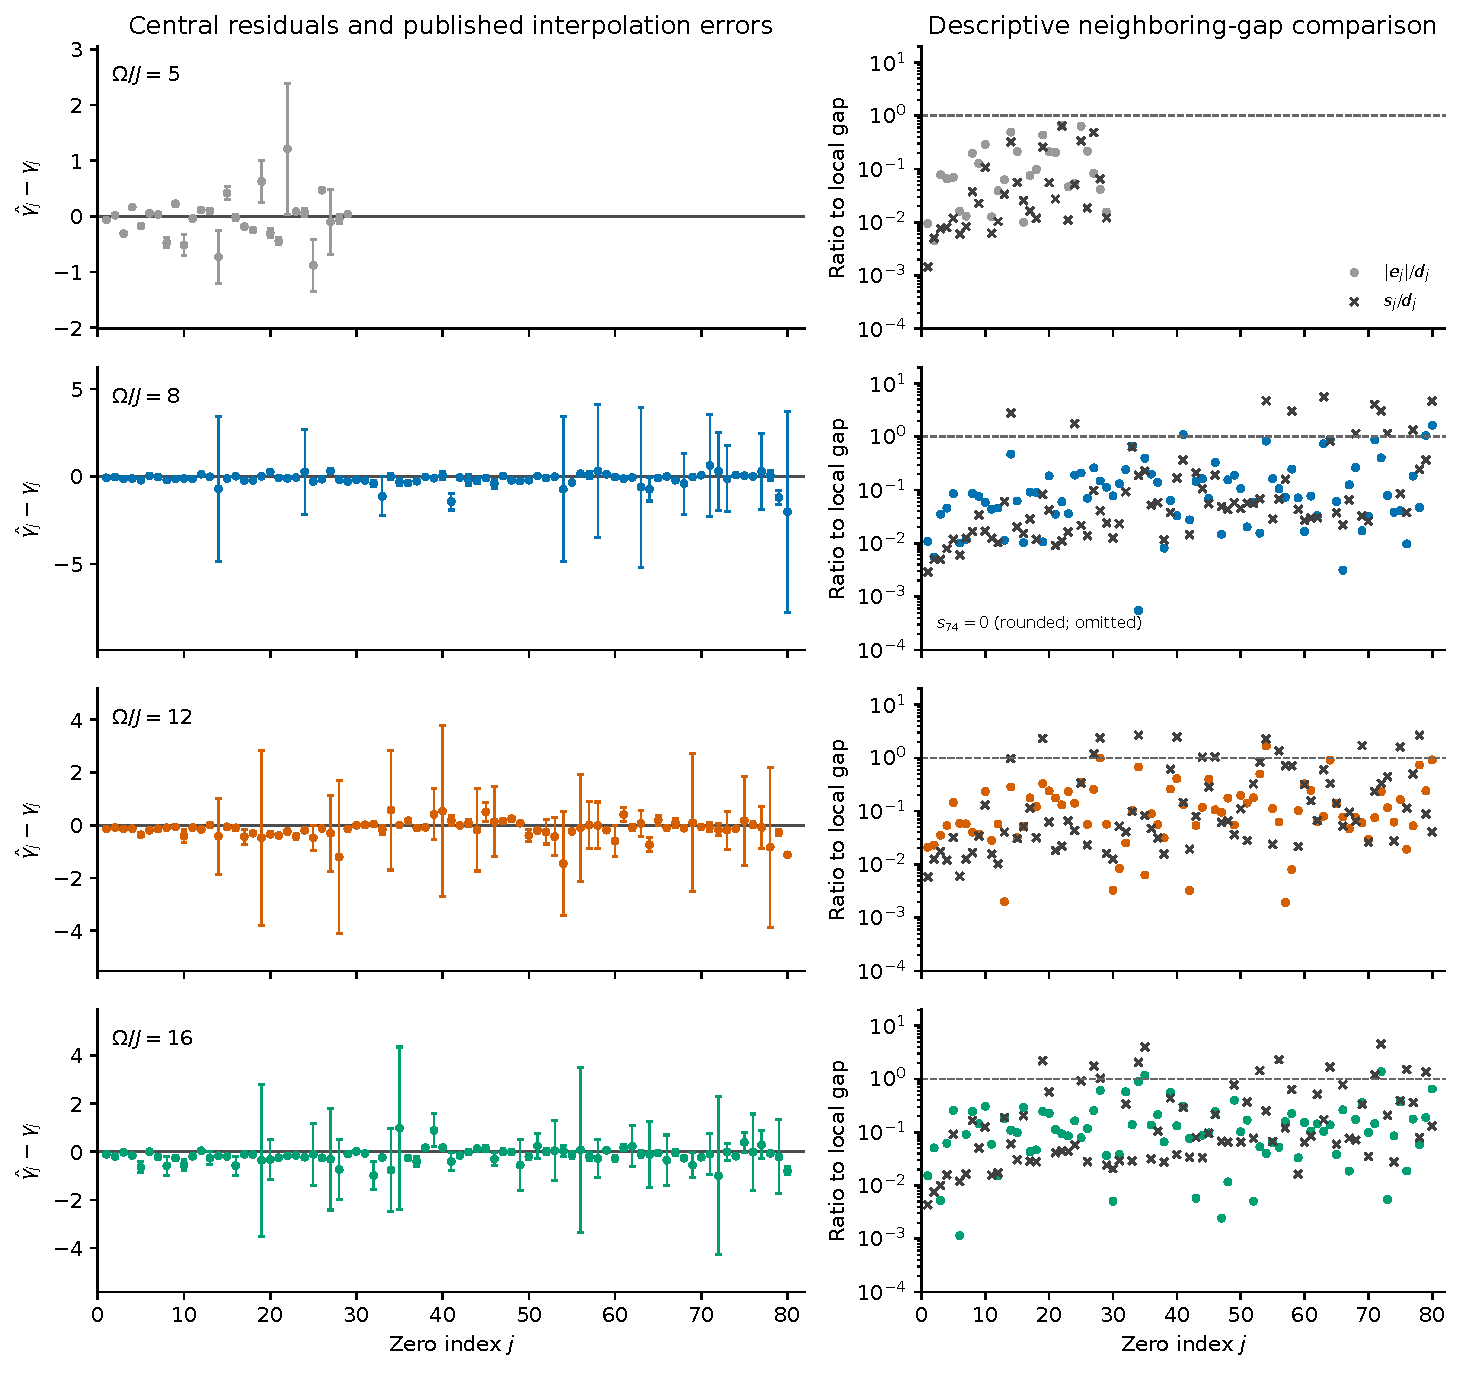
\includegraphics[width=.96\textwidth]{he2021_precision.pdf}
\caption{Reanalysis of He et al.'s supplementary tables \cite{He2021}. Left: residuals with published interpolation error bars, with independent vertical ranges so that all error bars remain visible. Right: central-residual and interpolation-error ratios to the smaller neighboring mathematical gap. The dashed line marks a ratio of one, not an experimentally validated threshold. A rounded-zero interpolation error at $j=74$, $\Omega/J=8$ is omitted only from the logarithmic right panel. The shorter $\Omega/J=5$ series contains 29 estimates. No cosmic component is fitted.}
\label{fig:ion}
\end{figure}

\subsection{A recent nuclear-spin implementation adds a different protocol}
Figure~\ref{fig:nmr} redraws the processed 2026 experiment. The target model defines an encoded evolution coordinate
\begin{equation}
 u=\varepsilon_0\tau_{\rm model}/\hbar,
\end{equation}
where $\varepsilon_0$ is the target Hamiltonian's energy scale and $\tau_{\rm model}$ its physical-time coordinate. Shaped control pulses implement the corresponding simulated evolutions; the plotted coordinate need not equal actual pulse duration. It is not cosmic age. The hardware data probe the first five zero neighborhoods. The reported root estimates $14.12$, $20.96$, $25.09$, $30.44$, and $32.93$ have residuals approximately $-0.0147$, $-0.0620$, $+0.0791$, $+0.0151$, and $-0.0051$ relative to the mathematical reference values. Their root-location uncertainties are not supplied, so we do not construct error bars or a weighted cross-platform accuracy ranking for these five numbers.

The same paper presents numerical demonstrations near much higher-index zeros, including index $10^{12}$. Those demonstrations must not be counted as hardware measurements. Nor can the 2021 count of 80, the 2026 hardware count of five, and a numerical index of $10^{12}$ be assembled into a time series of improving cosmic accessibility. They represent different encodings, tasks, and resource budgets. The time and inverse-temperature scans also have different central coherence magnitudes and are separate runs, so we do not pool their minima into a putative noise floor. Our use of the 2026 work is restricted to its finite-system observations and public processed data; it does not endorse a proof of RH, a universal thermodynamic interpretation, or a computational advantage from gate counts alone.

\begin{figure}[htbp]
\centering
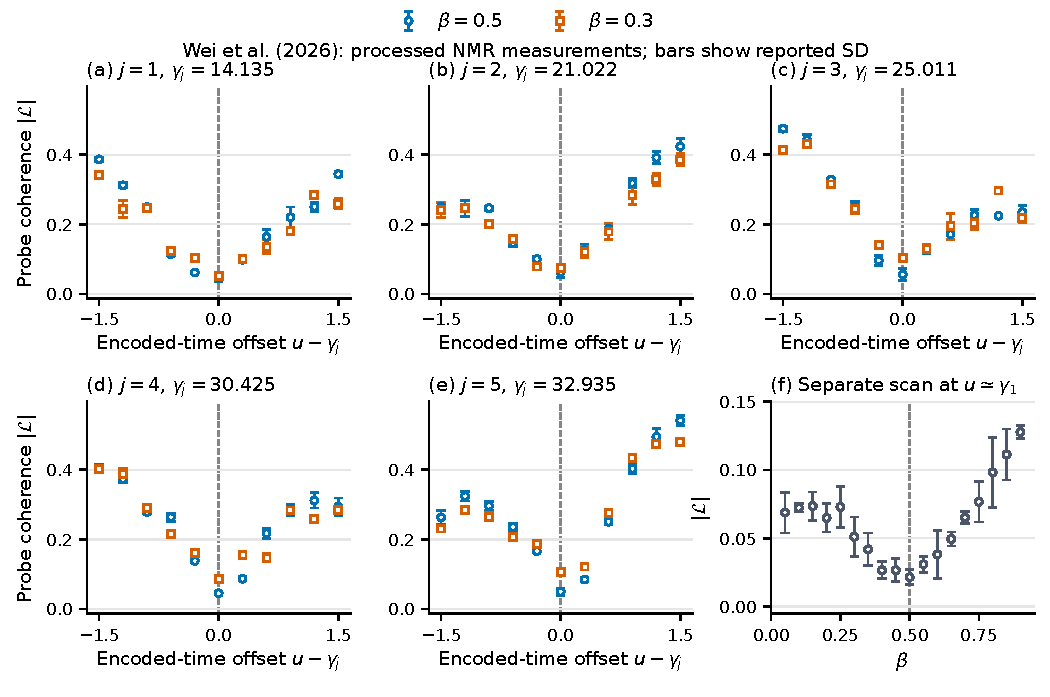
\includegraphics[width=\textwidth]{wei2026_experiment.pdf}
\caption{Public processed nuclear-spin data associated with Wei et al. \cite{Wei2026}, redrawn from the pinned author repository. The first five panels compare the reported probe-coherence magnitude near mathematical reference ordinates at two inverse temperatures; the final panel shows the inverse-temperature scan near the first zero. Bars reproduce supplied standard deviations of the processed observable. They are not uncertainties of estimated zero locations. The coordinate is the dimensionless laboratory encoding, not cosmic time. No high-index numerical demonstration is plotted as experimental data.}
\label{fig:nmr}
\end{figure}

\section{What a finite-resource zero estimate means}
\label{sec:operational}

The empirical distinction between a central residual and a reported
interpolation error motivates a definition based on a complete measurement
protocol. Nothing in this observational definition makes the mathematical
ordinate $\gamma_j$ evolve with cosmic time.

A protocol $\mathcal P$ specifies an encoding, a measured signal, a likelihood
$p(y\mid\theta,\boldsymbol\eta,\mathcal P)$, an estimator, and resources
such as interrogation duration, repetitions, bandwidth, and calibration.
Here $\theta$ is an unknown signal coordinate and $\boldsymbol\eta$ denotes
nuisance parameters. The ideal encoding places the relevant signal feature
at $\theta=\gamma_j$. For a tolerance $\Delta_j>0$ and a chosen error
probability $\epsilon_{\rm conf}$, a pointwise operational requirement is
\begin{equation}
 \Pr_{\mathcal P}\!\left(
   |\widehat\gamma_j-\gamma_j|\leq\Delta_j
 \right)\geq 1-\epsilon_{\rm conf}.
 \label{eq:accessible_criterion}
\end{equation}
Coverage must be justified over the declared nuisance-parameter range, not
only at a fitted calibration value. The tolerance may be absolute or relative
to a specified neighboring gap, but the choice must precede the comparison.
An uncertainty bar without its coverage and systematic-error model does not
establish Eq.~\eqref{eq:accessible_criterion}.

Inference in this definition uses the measured response. Returning a known
ordinate from a table is excluded as an independent analog measurement.
For a validation experiment, blinded signal coordinates or held-out target
windows can prevent reference information from being counted as experimental
precision. Engineered responses remain useful tests of control and encoding,
even when their construction already uses a mathematical function.

For a resource budget $\mathbf R$, let $\mathcal A(\mathbf R)$ contain the
targets meeting Eq.~\eqref{eq:accessible_criterion} in the declared protocol
class. An isolated-target height is
$T_{\rm target}=\sup\{\gamma_j:j\in\mathcal A(\mathbf R)\}$.
A complete-prefix requirement is stronger: one jointly budgeted procedure
must estimate every target through $J$, with simultaneous coverage
\begin{equation}
 \Pr\!\left(\bigcap_{j=1}^{J}
  \{|\widehat\gamma_j-\gamma_j|\leq\Delta_j\}\right)
 \geq1-\epsilon_{\rm conf}.
 \label{eq:prefix_coverage}
\end{equation}
The corresponding height is $\gamma_J$. Pointwise coverage does not imply
this joint guarantee, and isolated successful estimates need not form a
contiguous prefix. A scan ending at its largest reported target therefore
does not measure a fundamental maximum height.

\subsection{An illustrative quantum precision calculation}

Consider the frequency encoding $\omega=\kappa\theta$, where $\kappa$ has
units of inverse time. An initially equatorial qubit evolves under
\begin{equation}
 H_\theta=\frac{\hbar\kappa\theta}{2}\sigma_z,
 \qquad U_\theta(\tau)=\exp(-i\kappa\theta\tau\sigma_z/2).
\end{equation}
The quantum Fisher information per ideal independent interrogation is
$F_Q=(\kappa\tau)^2$. Under the regularity and local unbiasedness assumptions
of the quantum Cram\'er--Rao framework, $M$ independent trials obey
\begin{equation}
 \operatorname{Var}(\widehat\theta)
 \geq\frac{1}{M F_Q}
 =\frac{1}{M\kappa^2\tau^2}.
 \label{eq:ramsey_qfi}
\end{equation}
This is an elementary example within quantum estimation theory
\cite{BraunsteinCaves1994,Giovannetti2006}, not a universal noise model for
every Riemann-zero implementation. For a binary Ramsey signal
$p_+=[1+V\cos(\kappa\theta\tau+\phi)]/2$ with known, parameter-independent
visibility $V$, operation at quadrature gives classical Fisher information
$F=V^2(\kappa\tau)^2$ per shot. Its local statistical bound becomes
$\sigma_\theta\geq1/(V\kappa\tau\sqrt M)$.

A lower bound is not an achieved uncertainty or a coverage guarantee.
Bias, uncertain visibility, correlated shots, and calibration require their
own model. Moreover, the phase is periodic: local Fisher information does
not resolve global aliases without additional interrogation times or prior
range information. A finite-window Fourier width of order $2\pi/\tau$
likewise does not establish a universal prohibition on more precise parameter
estimation; protocols using quantum sensing or external synchronization can
change the relevant resolution behavior \cite{Gefen2019,Boss2017}.
Finite precision follows here from a specified finite-information
experiment under specified assumptions; it does not prove a nonzero error
floor shared by every physically possible protocol.

\subsection{Mean density as a conditional illustration}

The smooth Riemann--von Mangoldt count is
\begin{equation}
 \overline N(T)=\frac{T}{2\pi}\log\frac{T}{2\pi}
 -\frac{T}{2\pi}+\frac78,
 \qquad
 \overline d(T)\simeq\frac{2\pi}{\log(T/2\pi)}.
 \label{eq:mean_spacing}
\end{equation}
The second expression describes the asymptotic mean spacing, not the smallest
individual gap. If a working model supplies an achieved, dimensionless
resolution scale $\delta$ and uses the illustrative criterion
$\delta\leq q\overline d(T)$, with prescribed $0<q<1$, its crossover is
\begin{equation}
 T_{\rm env}=2\pi\exp\!\left(\frac{2\pi q}{\delta}\right).
 \label{eq:mean_envelope}
\end{equation}
This is a mean-density illustration in the asymptotic regime. It is neither
an apparatus-independent bound nor a statement that all lower zeros are
resolvable. It assumes a usable resolution scale rather than substituting a
Cram\'er--Rao lower bound as if it were attained. Bandwidth, signal amplitude,
individual gaps, and calibration may restrict the experiment first. A
conversion from an RMS error to a confidence tolerance additionally requires
a probability model. The exponential sensitivity of
Eq.~\eqref{eq:mean_envelope} makes an absolute height forecast especially
unstable without these ingredients.

\section{A conditional cosmic-time extension}
\label{sec:cosmic_extension}

\subsection{Motivation from the published dynamical model}

The recently published numerical study of a non-autonomous quadratic map
\cite{Wang2026Spectral} investigates a schedule of the form
\begin{equation}
 x_{n+1}=1-\lambda_n x_n^2,
 \qquad
 \lambda_n=\mu_c+\frac{k_1}{\log^2n}
                  +\frac{k_2}{\log^3n},\qquad n>1.
 \label{eq:published_map}
\end{equation}
Its leading inverse-log-squared term is a heuristic numerical ansatz. The
motivation combines the known logarithmic spectral density with an assumed
square-root response of an eigenphase spacing to a structural perturbation.
The resulting transfer-operator correspondence is not a demonstrated
isomorphism or a self-adjoint Hilbert--P\'olya Hamiltonian. The paper reports
larger out-of-sample errors and local spacing statistics inconsistent with
GUE, so its global spectral correspondence is not evidence of matching every
statistical property of the zeta zeros.

Two further assumptions are required to use this motivation here: a mapping
from iteration or spectral scale to cosmic age, and a response law connecting
the evolving structural parameter to a measured precision scale. Neither is
supplied by the numerical correspondence. In particular, preserving the
power two in a noise amplitude assumes a suitable response relation; it
does not follow solely from copying the map schedule.

We therefore introduce the separately testable candidate
\begin{equation}
 \delta_{\rm c}(t)=\delta_{{\rm c}0}
 \left[\frac{\log(t_0/t_*)}{\log(t/t_*)}\right]^p,
 \qquad t>t_*,\quad \delta_{{\rm c}0}\geq0,
 \label{eq:cosmic_ansatz}
\end{equation}
with $p=2$ as the primary hypothesis. Here $\delta_{\rm c}$ is a proposed
contribution to the standard deviation of an encoded ordinate estimator,
not a change in the mathematical ordinate. The scale $t_*$ makes the logarithm
dimensionless, and $t_0$ is a normalization epoch. The amplitude and transfer
to a particular apparatus are not fixed by the earlier map coefficients.
The case $\delta_{{\rm c}0}=0$ is a permitted null model. Neither the
singularity at $t=t_*$ nor an extrapolation into that regime is claimed to
describe early-universe physics.

For a fixed estimator and protocol, one possible phenomenological error
model is
\begin{equation}
 \operatorname{MSE}(\widehat\gamma_j)
 =b_j^2+\sigma_{{\rm stat},j}^2+\sigma_{{\rm cal},j}^2
  +\delta_{{\rm c},j}^2(t).
 \label{eq:conditional_budget}
\end{equation}
This decomposition assumes that the three random error components have zero
mean and are mutually uncorrelated; $b_j$ is the remaining bias. Correlations
require covariance terms. Calibration uncertainty is not automatically
independent random noise, and $\delta_{{\rm c},j}$ may differ across encodings.
Calling it a floor further assumes that the specified component survives
the averaging and control operations allowed by the protocol. Independent
per-shot noise instead decreases on repetition; a correlation model is
needed before asserting an irreducible floor.

For $\delta_{{\rm c}0}>0$, Eq.~\eqref{eq:cosmic_ansatz} gives
\begin{equation}
 \frac{d\log\delta_{\rm c}}{dt}
 =-\frac{p}{t\log(t/t_*)}.
 \label{eq:cosmic_derivative}
\end{equation}
As a scale illustration, choose $t_0=13.8\,\mathrm{Gyr}$ and
$t_*=5.391247\times10^{-44}\,\mathrm{s}$, a conventional Planck-time-scale
normalization rather than an inferred parameter. Using a Julian year,
$\log(t_0/t_*)=140.24423$. For $p=2$, the present fractional rate is
$-1.0334\times10^{-12}\,\mathrm{yr}^{-1}$, corresponding to approximately
$-5.17\times10^{-13}$ in half a year. This is the fractional change of the
hypothesized component, not an observed drift or the fractional change of
the total experimental uncertainty. Its amplitude remains unspecified.

\subsection{Resource growth, identifiability, and falsification}

Let $\mathfrak P(t)$ be the feasible set of protocols including their
calibrated performance at age $t$. If
$\mathfrak P(t_1)\subseteq\mathfrak P(t_2)$ for $t_2>t_1$, with the same
target and confidence criterion, optimization over these sets makes either
accessible-height definition nondecreasing. This is a conditional consequence
of set inclusion. Cosmic age alone does not establish the inclusion:
usable energy, causal access, coherence, and calibration stability need not
improve monotonically. Even in Eq.~\eqref{eq:conditional_budget}, a decreasing
cosmic component does not improve the total error if other components grow.

Entropy and energy limits motivate explicit resource accounting
\cite{Bekenstein1981,MargolusLevitin1998,Lloyd2002}. Converting them into a
zero-height limit would additionally require an encoding, a task definition,
and a justified computational or measurement cost. An explicit table of $J$
values at $b$ bits per value requires roughly $Jb$ bits; an algorithm plus an
index may be far shorter. Finite storage therefore does not by itself select
a largest zero index. The rigorous interval-arithmetic verification of RH
through ordinate $3\times10^{12}$ \cite{PlattTrudgian2021} is a separate
category of evidence from analog spectroscopy, but rules out interpreting
an ordinate of order $4200$ as a general limit on physically computable
zero information.

The available experiments provide no controlled comparison of the same
calibrated apparatus at substantially different cosmic ages. Within each
dataset, changing the zero index or a drive parameter does not vary cosmic
age. A single-epoch residual budget generally cannot identify
$\delta_{{\rm c}0}$ separately from unknown calibration and model discrepancy,
and it cannot select $p=2$ over a constant or another slow time dependence.
Publication dates do not constitute an aging series.

A discriminating test would first fix the encoding, estimator, nuisance
model, and allowed averaging operations, then check the resource dependence
on held-out targets. Repeated independently calibrated measurements could
test the signed drift in Eq.~\eqref{eq:cosmic_derivative}, provided a
nonzero component and sufficient sensitivity were established. A specified
positive-amplitude model could be excluded by a sufficiently stringent
upper limit or by incompatible drift or resource scaling. The unrestricted
family allowing arbitrarily small amplitude cannot be ruled out by a finite
null result. Poor estimates, improved estimates, and null drift must not all
be treated as confirmation of cosmic aging.


\section{Conditional numerical illustrations}
Figure~\ref{fig:resources} illustrates the difference between a resource model and a measurement of cosmic evolution. In panel (a), we assume an attained dimensionless error scale
\begin{equation}
 \delta(M)=\sqrt{M^{-1}+b^2}
\end{equation}
and compare it with one quarter of the asymptotic mean spacing. The normalization corresponds to unit $\kappa\tau V$ in a locally efficient Ramsey example. The floors $b=0,0.1,0.3$ are chosen for illustration; none is estimated from either experiment. Solving $\delta=\overline d(T)/4$ produces an exponentially sensitive mean-density envelope. The very large values in the zero-floor curve demonstrate the incompleteness of a density-only criterion: finite bandwidth, signal preparation, global identifiability, local gap fluctuations, and calibration have not been imposed. This curve is not a forecast of an achievable experiment.

Panel (b) shows normalized logarithmic aging with exponents $p=1,2,3$, at fixed illustrative $t_0=13.8$ Gyr and $t_\ast=5.391247\times10^{-44}$ s. The $p=2$ curve represents the proposed form; the alternatives show that monotonic evolution alone does not select it. The amplitude is uncalibrated, and normalization at $t_0$ is not a fit. Even across the broad interval 1--100 Gyr the normalized curves vary slowly. Over half a year the $p=2$ scale changes by only about $-5.17\times10^{-13}$ fractionally under these assumptions. Recent publication of a new experiment therefore provides new protocol information, rather than a useful cosmic-aging baseline by itself.

\begin{figure}[htbp]
\centering
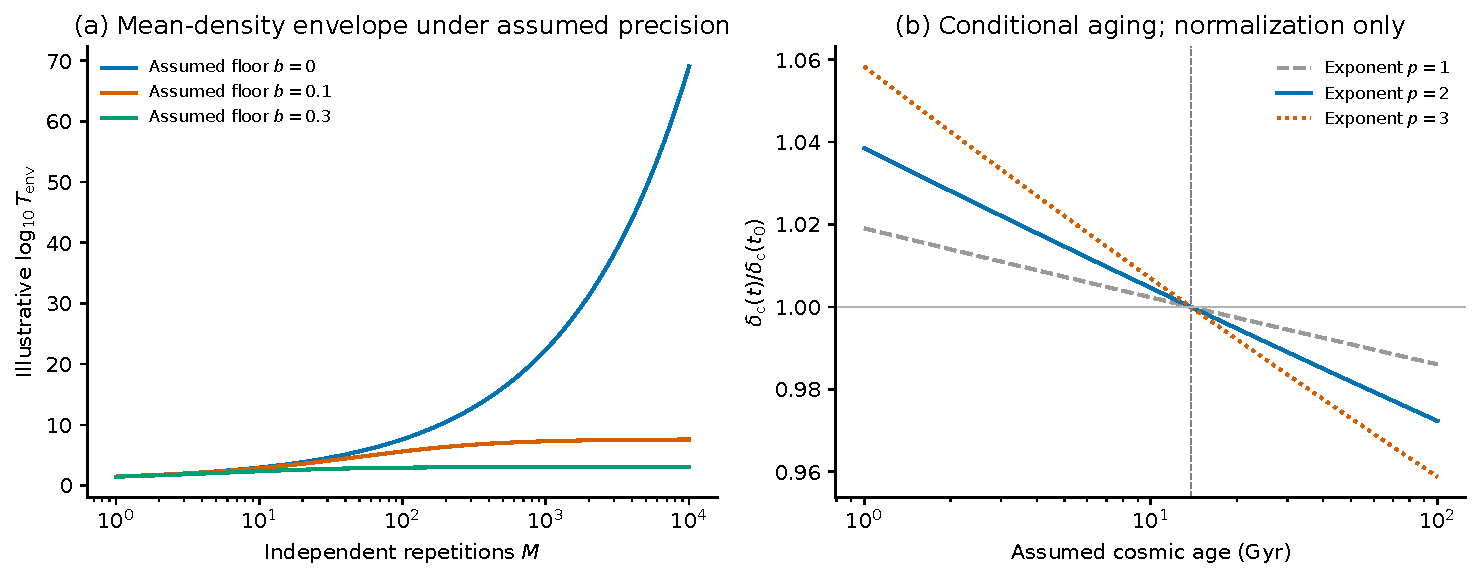
\includegraphics[width=\textwidth]{conditional_resources.pdf}
\caption{Conditional scenarios, with no experimental parameter fit. (a) Mean-density envelope obtained from an assumed attained precision, a one-quarter spacing criterion, and illustrative error floors. It does not impose local gaps, bandwidth, or global identification costs. (b) Normalized candidate cosmic uncertainty scales with exponents $p=1,2,3$. The vertical line is the chosen normalization age of 13.8 Gyr; the scale $t_\ast$ is a convention for this illustration. The two panels do not constitute a calibration of a cosmic zero-height ceiling.}
\label{fig:resources}
\end{figure}

Figure~\ref{fig:heatmap} presents the same resource model as a two-dimensional landscape. Increasing repetitions moves a protocol to the right; reducing its assumed floor moves it downward. The dashed crossover $b=M^{-1/2}$ separates statistical-term and floor dominance. The three stars are chosen scenarios, not laboratory or cosmological calibration points. Their progression shows why collecting more samples alone eventually provides little benefit when the floor remains fixed, while a smaller floor can change the illustrative envelope much more strongly. The color represents $\log_{10}T_{\rm env}$ rather than a zero index, and the displayed grid is not clipped. As in Fig.~\ref{fig:resources}, this landscape illustrates a mean-spacing criterion without imposing the other requirements for an attainable experiment.

\begin{figure}[htbp]
\centering
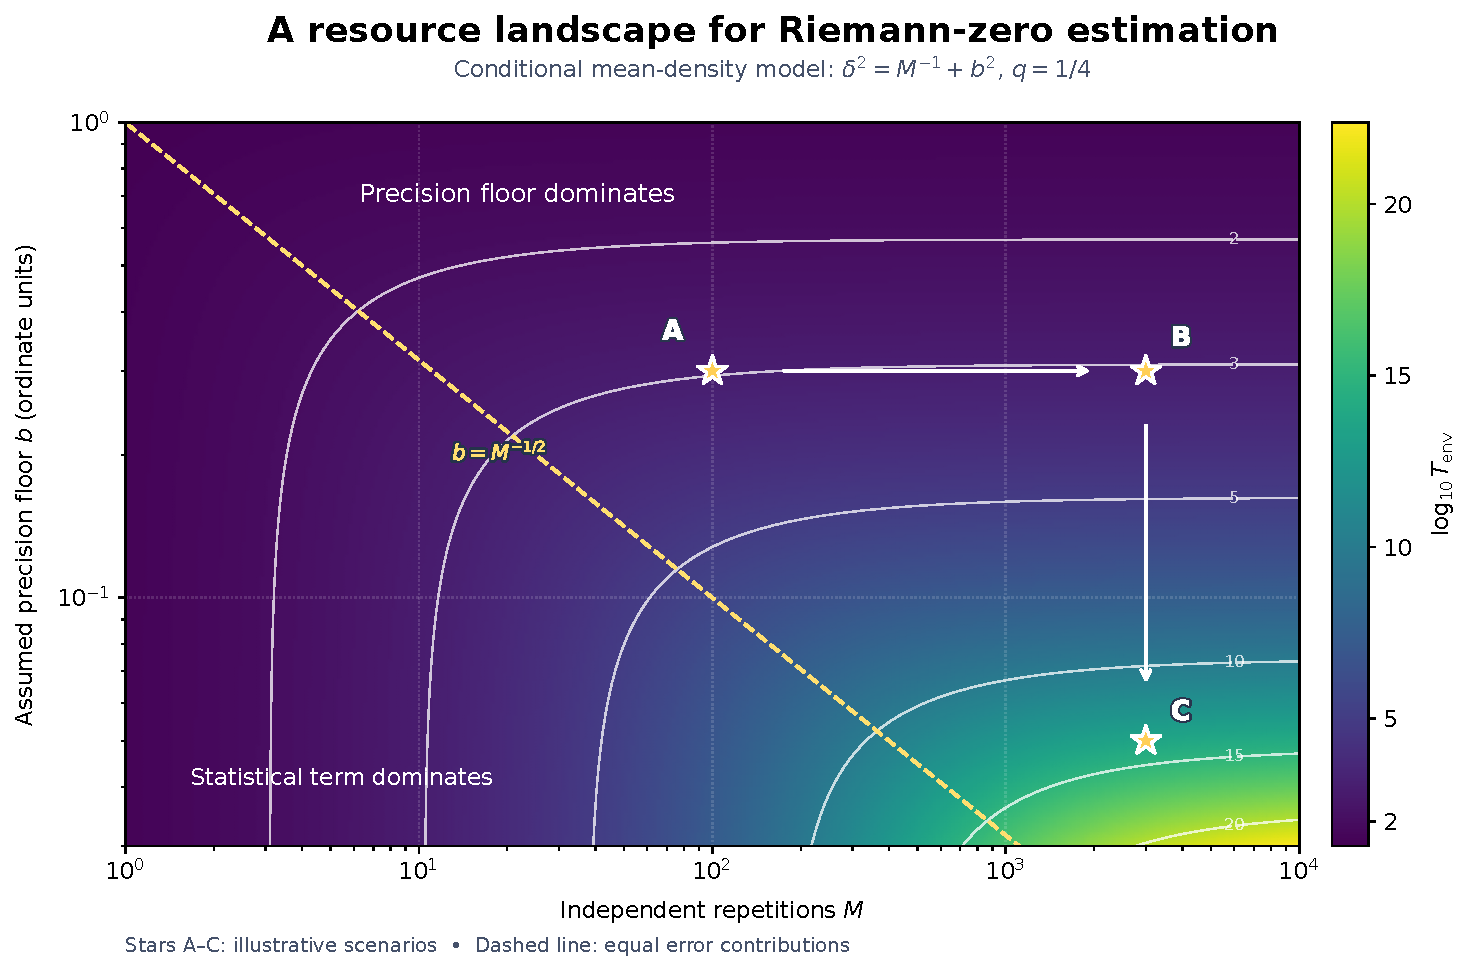
\includegraphics[width=\textwidth]{resource_precision_heatmap.pdf}
\caption{Conditional resource--precision heatmap for $\delta^2=M^{-1}+b^2$, $\kappa\tau V=1$, and $q=1/4$. Color and white contour labels show $\log_{10}T_{\rm env}$ from Eq.~\eqref{eq:mean_envelope}; they do not count zeros. The dashed line marks equal statistical and floor contributions. Stars A, B, and C correspond respectively to $(M,b)=(100,0.3)$, $(3000,0.3)$, and $(3000,0.05)$. The arrows show two possible parameter changes. Small-ordinate colors are formal extrapolations of the asymptotic approximation. Both the grid and the stars are illustrative, with no fit to an experiment and no identified cosmic cutoff.}
\label{fig:heatmap}
\end{figure}

\section{Existing astronomical spectra and a data-informed observing outlook}
\label{sec:highz}
\subsection{An empirical pilot from public absorption spectra}
High-redshift spectroscopy can sample material at earlier cosmic epochs without waiting for a measurable change during a laboratory lifetime. The relevant information would be a physical imprint formed at emission or absorption, however, not the precision available to an observer living at that epoch. A change only in an observer's computational resources need not leave such an imprint. We therefore analyze existing spectra as a test of data quality and inference requirements, without treating them as measurements of Riemann zeros.

The UVES Spectral Quasar Absorption Database, SQUAD DR1, contains 467 final quasar spectra \cite{Murphy2019SQUAD}. We downloaded two historical coadded products: HE\,0515$-$4414, with a reference absorber at $z_{\rm abs}=1.1508$, and Q0347$-$3819, also catalogued as Q0347$-$383, at $z_{\rm abs}=3.025$. Their emission redshifts, 1.710 and 3.205, are different quantities. The decoded files contain 279,787 and 241,828 source-valid pixels, respectively, on vacuum heliocentric wavelength grids with native sampling of $1.3\,\mathrm{km\,s^{-1}}$. The contributing exposures date from 1999--2009; retrieval in 2026 is not a new observing epoch. These two convenience examples are a development sample, not a homogeneous redshift survey.

We use archived NIST ASD Ritz wavelengths to establish consistent velocity coordinates \cite{NISTASD2024}. The six Fe\,II transitions near 1608, 2344, 2374, 2382, 2586, and 2600\,\AA\ share a lower level but do not form a complete, symmetry-resolved sequence of adjacent eigenvalues. Their spacing is consequently not a direct GUE or zero-truncation observable. Precise laboratory wavelengths and the treatment of isotope structure are separate requirements for transition-frequency inference \cite{MurphyBerengut2014}.

Figure~\ref{fig:highz_profiles} and Table~\ref{tab:highz_observed} report measurements made directly from the archived flux, rather than injected profiles. We define the rest-frame equivalent width and flux-deficit centroid within a stated interval by
\begin{align}
 W_r&=\frac{\lambda_0}{c}\sum_i(1-F_i)\Delta v_i,\\
 \bar v&=\frac{\sum_i\widetilde v_i(1-F_i)\Delta v_i}
                  {\sum_i(1-F_i)\Delta v_i}.
 \label{eq:profile_moments}
\end{align}
Here $F_i$ is continuum-normalized flux, $\Delta v_i$ is the portion of the native pixel inside the interval, and $\widetilde v_i$ is the midpoint of that portion. Flux above the continuum contributes with its sign; we do not clip negative absorption. The HE interval is $[-25,110]\,\mathrm{km\,s^{-1}}$ and the Q0347 interval is $[-80,35]\,\mathrm{km\,s^{-1}}$, relative to the stated absorber redshifts. These common-within-sightline intervals were chosen after inspecting the profiles and are exploratory. They are not integrations over the full absorption systems.

The tabulated errors propagate the archived pixel errors with fixed continuum and wavelength calibration and a diagonal covariance approximation. We also propagate the separately supplied expected-fluctuation array and test assumed pixel correlations. Neither array supplies the complete covariance or systematic error budget. Near-zero or negative flux is retained in flux integrals but is not converted into a supposedly precise apparent optical depth or column density; unresolved saturation and noise require additional treatment \cite{SavageSembach1991,Fox2005AOD}.

\begin{table}[htbp]
\caption{Measurements of actual finite-window absorption profiles. Errors are conditional diagonal statistical $1\sigma$, not complete physical-frequency uncertainties. $\Delta_C$ is the maximum absolute centroid change under a prescribed $\pm1\%$ continuum perturbation; $\Delta_W$ is the maximum change under the stated $10\,\mathrm{km\,s^{-1}}$ boundary variations. These sensitivities are not random error bars. The high-redshift red windows are omitted from this science-oriented table because of contamination or low signal-to-noise; their screening integrals remain in the data release. HE entries remain subject to blend and saturation review.}
\label{tab:highz_observed}
\centering
\small
\setlength{\tabcolsep}{5pt}
\begin{tabular}{llrrrr}
\toprule
Sightline & Fe II & $W_r$ (m\AA) & $\bar v$ (km/s) & $\Delta_C$ (km/s) & $\Delta_W$ (km/s) \\
\midrule
HE 0515 & 1608 & $179.20\pm0.50$ & $33.883\pm0.117$ & 0.363 & 1.026 \\
HE 0515 & 2344 & $506.05\pm0.35$ & $35.306\pm0.031$ & 0.153 & 1.066 \\
HE 0515 & 2374 & $220.84\pm0.44$ & $33.871\pm0.083$ & 0.439 & 0.811 \\
HE 0515 & 2382 & $757.11\pm0.26$ & $35.607\pm0.018$ & 0.099 & 1.660 \\
HE 0515 & 2586 & $442.98\pm0.38$ & $34.623\pm0.037$ & 0.213 & 0.978 \\
HE 0515 & 2600 & $777.27\pm0.31$ & $35.346\pm0.020$ & 0.109 & 1.585 \\
Q0347 & 1608 & $235.57\pm0.65$ & $-20.194\pm0.108$ & 0.062 & 1.260 \\
\bottomrule
\end{tabular}

\end{table}

\subsection{Observed profile sensitivity limits the interpretation of small errors}
The HE profile-centroid statistical errors span $18$--$117\,\mathrm{m\,s^{-1}}$. Prescribing a $1\%$ continuum perturbation changes the same descriptors by $99$--$439\,\mathrm{m\,s^{-1}}$, while changing integration boundaries by $10\,\mathrm{km\,s^{-1}}$ changes them by $0.81$--$1.66\,\mathrm{km\,s^{-1}}$. The perturbations have not been measured as actual continuum errors, and changing the interval can include different gas components. Their purpose is to show that an integrated absorption centroid is not automatically an atomic transition-frequency estimator. In the HE 2382 and 2600 windows, respectively, approximately $36.2\%$ and $31.7\%$ of pixels have $F<0.1$, motivating explicit saturation checks.

The high-redshift Fe\,II 1608 window gives $W_r=235.57\pm0.65$\,m\AA\ under the same conditional error convention. The 2344, 2374 and 2382 windows lie around $9435$--$9591$\,\AA\ and require telluric assessment. The 2586 and 2600 windows near $1.04\,\mu$m have full-window median continuum-to-error ratios of only 1.31 and 2.06 per native pixel. We retain their signed integrals for quality screening, but do not report usable scientific centroids from them. A statistically nonzero integral in a contaminated or low-quality window does not establish a clean identified transition.

\begin{figure}[htbp]
\centering
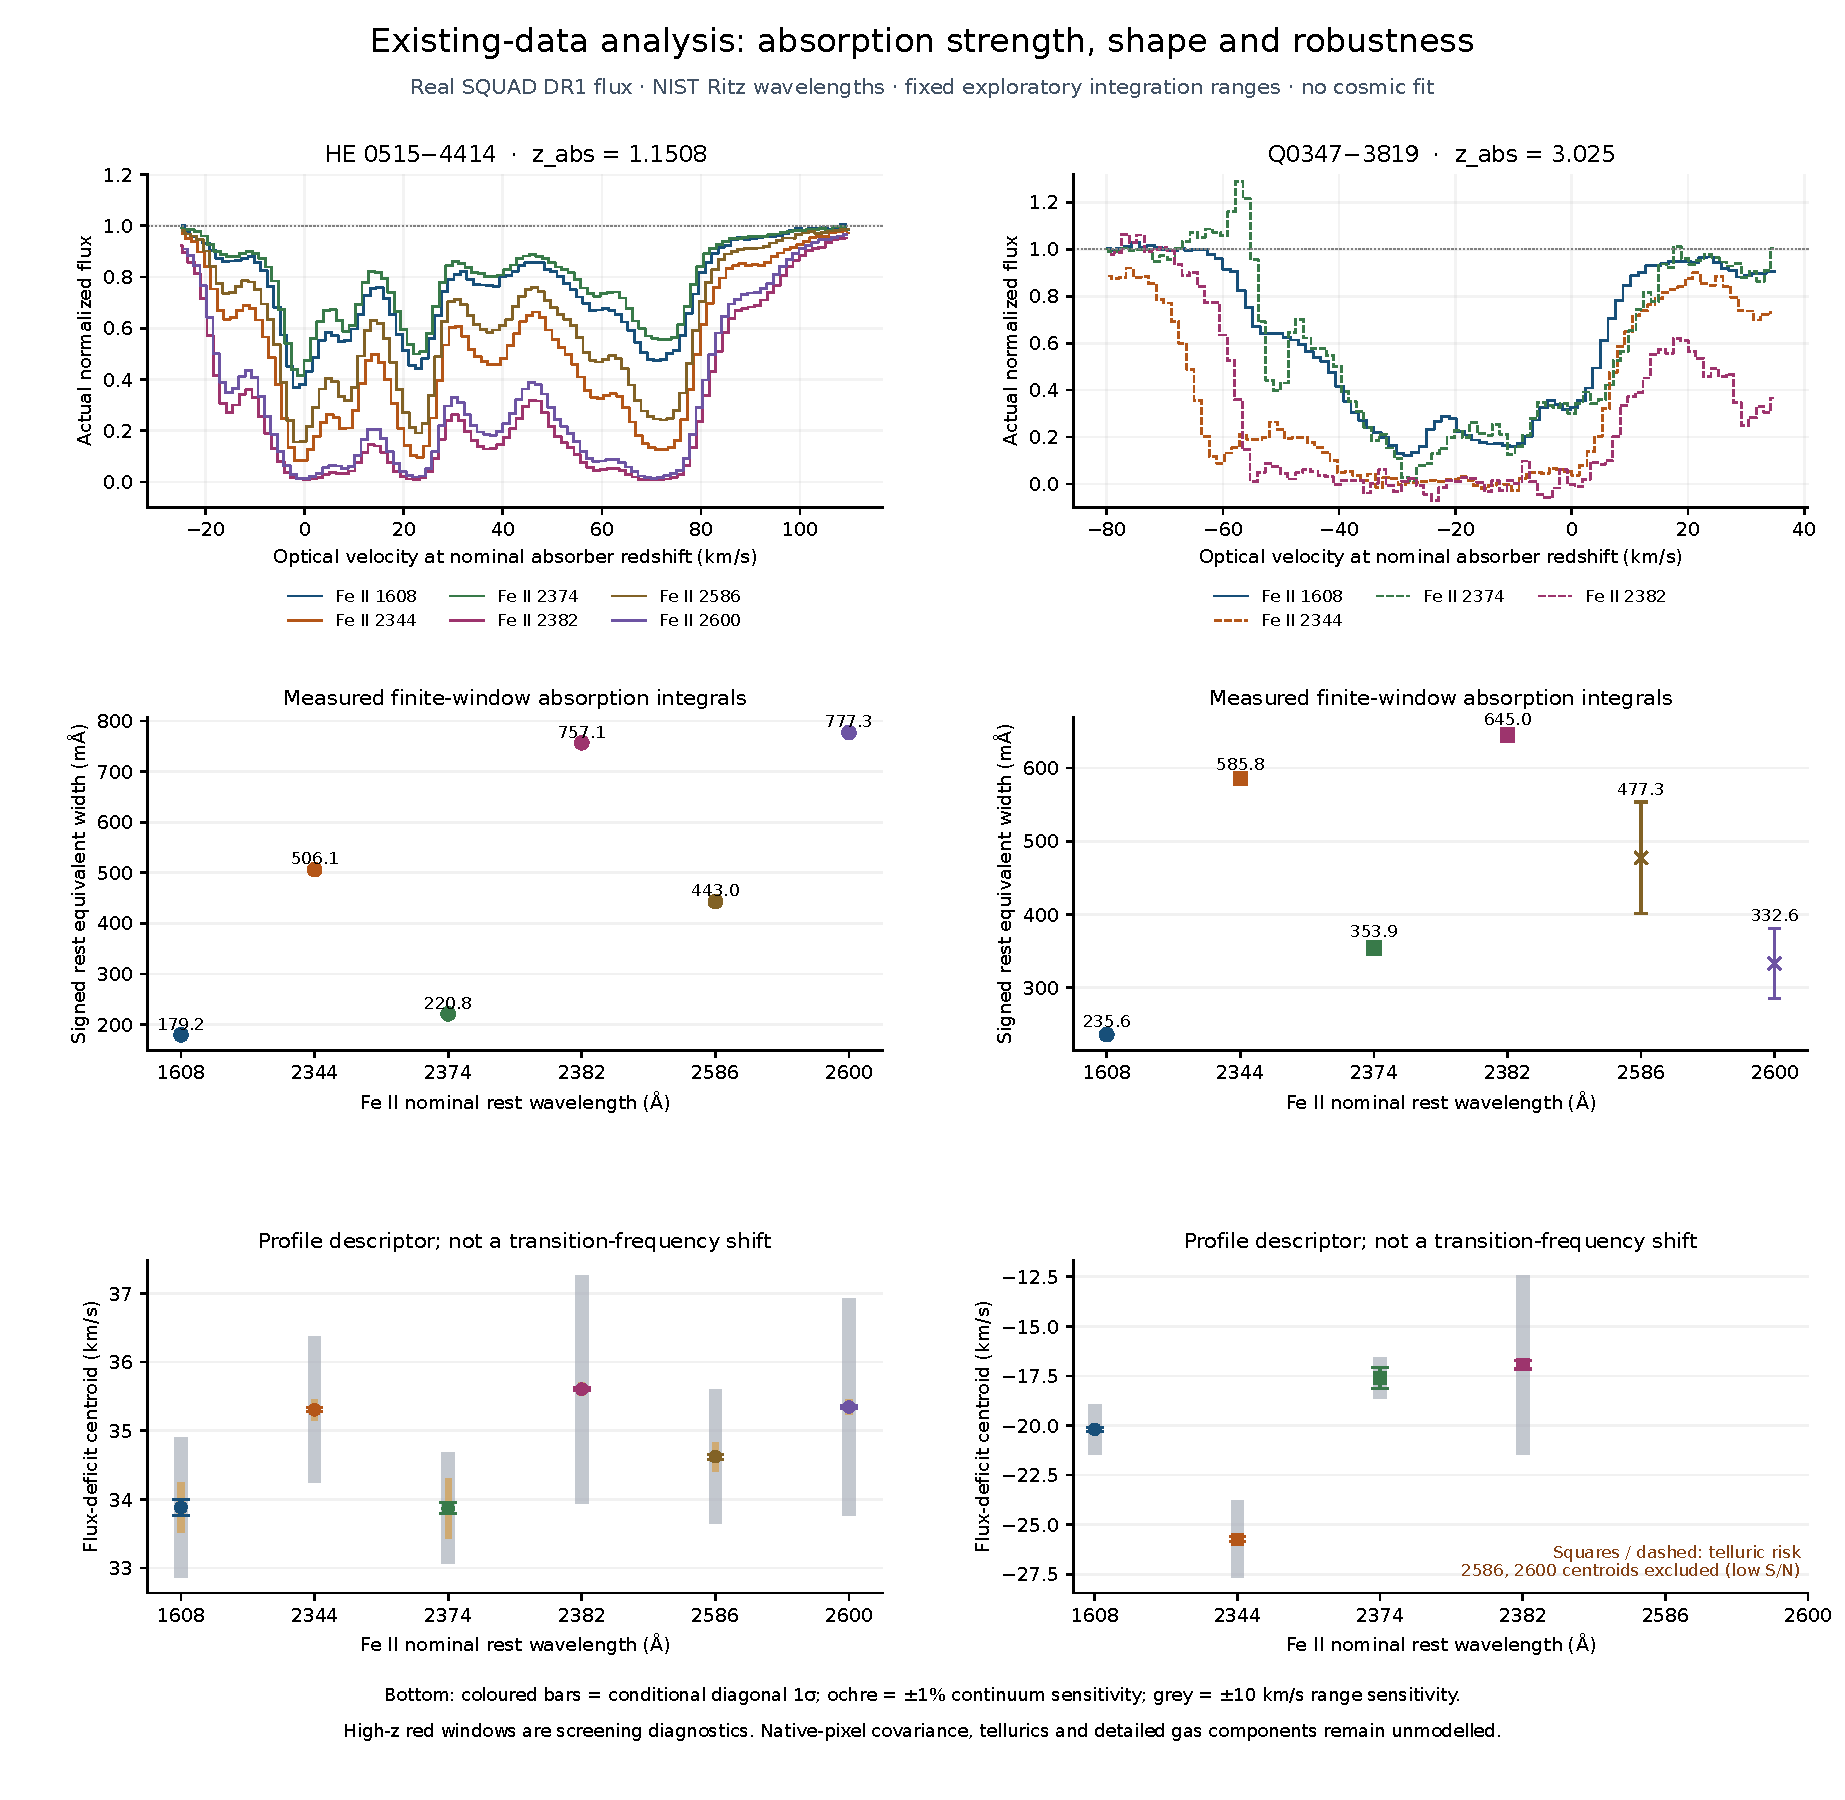
\includegraphics[width=.98\textwidth,height=.76\textheight,keepaspectratio]{highz_observed_profiles.pdf}
\caption{Actual SQUAD flux and finite-window measurements, using NIST Ritz wavelengths. Top: observed profiles. Middle: signed absorption integrals; high-redshift squares flag telluric risk and crosses flag low signal-to-noise. Bottom: absorption-centroid descriptors with conditional statistical errors and separate continuum and interval sensitivity ranges. The latter ranges are illustrative robustness diagnostics, not confidence intervals. No time-dependent physical parameter is fitted. Different line strengths and gas-component weightings can produce different descriptors without changing transition frequencies.}
\label{fig:highz_profiles}
\end{figure}

We further fit a descriptive registration model to actual HE flux, using Fe\,II 2374 as a noisy empirical template for 2586 and 2600:
\begin{equation}
 F_j^{\rm reg}(v)=[c_0+c_1v/(100\,\mathrm{km\,s^{-1}})]
                  F_{2374}(v-\delta)^a.
 \label{eq:registration}
\end{equation}
The shift $\delta$, depth transformation $a$, and continuum terms are fitted. Linear interpolation propagates template noise as well as target noise, and the approximate Gaussian objective includes the parameter-dependent log-variance term. Pixel and interpolation correlations are omitted. We compare affine-flux transformations, two error arrays and three velocity intervals; these are sensitivity analyses of the same data, not independent discoveries.

Using the source expected-fluctuation array, the full-interval 2586 power registration gives an offset of about $+17\,\mathrm{m\,s^{-1}}$ but a nominal diagonal residual statistic divided by degrees of freedom of 5.26. Restricting to $[40,95]\,\mathrm{km\,s^{-1}}$ gives about $-34\,\mathrm{m\,s^{-1}}$ and a ratio of 0.88. These offsets are registration descriptors, not estimates of a physical frequency drift. The whole-interval 2600 fit under the same error convention is substantially worse, with a ratio of about 34.2. Small curvature errors from such fits are not reliable accuracy claims; boundary solutions and interpolation-knot curvature are explicitly flagged, with the corresponding formal errors withheld.

This failure of a simple transformation is expected to be possible under conventional physics. In general, for an instrumental line-spread operator $L$,
\begin{equation}
 (L*e^{-\tau})^a\ne L*e^{-a\tau}.
\end{equation}
Moreover, additional absorption in Fe\,II 2586 is reported in both UVES and ESPRESSO observations of this absorber \cite{Murphy2022ESPRESSO}. For this UVES registration diagnostic, the published ESPRESSO exclusion mask has not been transferred to the SQUAD coadd, so these profiles retain the identified blend. The present registration is a stress test of a simplified model, not a replacement for exposure-level multicomponent line-profile analysis. Its useful result is the demonstrated need for that analysis before interpreting small fitted offsets.

\begin{figure}[htbp]
\centering
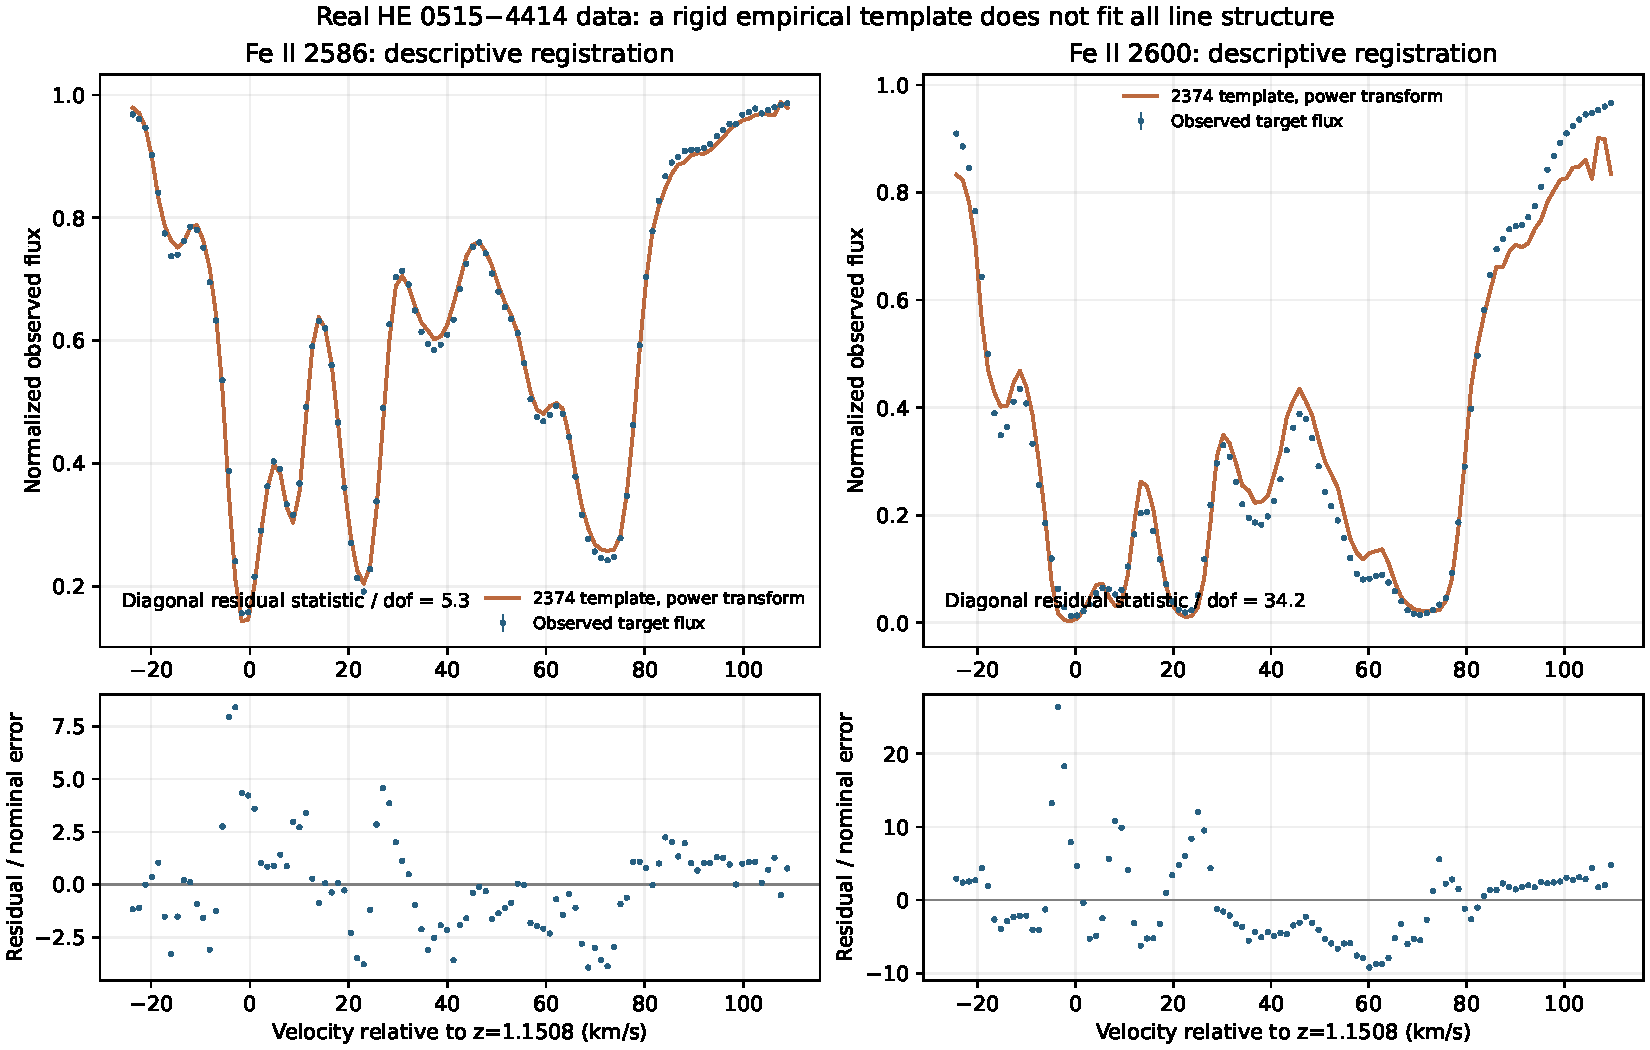
\includegraphics[width=.97\textwidth]{highz_observed_registration.pdf}
\caption{Descriptive fits to real HE\,0515$-$4414 data. Observed Fe\,II 2586 and 2600 flux is compared with a fitted power transformation of the observed 2374 template over the full selected interval. Lower panels show residuals divided by the nominal combined target/template error. The failures are diagnostics of this simplified transformation and profiles retaining the identified blend, not evidence for new physics. No physical shift uncertainty, cosmic amplitude or zero cutoff is inferred.}
\label{fig:highz_registration}
\end{figure}

\subsection{A joint physical baseline test with ESPRESSO}
\label{sec:espresso_null}
% Generated from selected fitted results; do not edit numbers manually.
\newcommand{\EspressoNullChi}{2305.49}
\newcommand{\EspressoNullNu}{2784}
\newcommand{\EspressoDeltaChi}{51.71}
\newcommand{\EspressoAdded}{5}

The descriptive registration above does not test whether ordinary absorption physics can explain the profiles. We therefore perform a separate joint Voigt-profile analysis of the public ESPRESSO spectrum of HE\,0515$-$4414 \cite{Murphy2022ESPRESSO}. We use six Fe\,II transitions, at 2260, 2344, 2374, 2382, 2586, and 2600\,\AA, in the published right region of the same $z\simeq1.1508$ absorber. These observations were acquired in 2018--2020; retrieval in 2026 is not new acquisition. Unlike the UVES set, this set includes weak 2260 but lacks 1608, which falls outside ESPRESSO coverage.

Our conventional hypothesis $H_0$ fixes laboratory transition-frequency relations, including $\Delta\alpha/\alpha=0$, and fits a common set of gas components to all six lines. Each of the 45 published Fe\,II components supplies a column density $N_k$, velocity $v_k$, and Doppler parameter $b_k$, all re-optimized here. The opacity of each transition is the sum of Voigt opacities, including the isotope wavelengths and abundance-weighted oscillator strengths in the authors' archived atomic input \cite{MurphyBerengut2014}. Absorption is exponentiated before instrumental convolution. For pixel $i$ of transition $j$, the model is
\begin{equation}
 m_{ji}=C_j(v_{ji})\left\{Z_j+(1-Z_j)\,
 \mathcal P_{ji}\!\left[L_j*\exp\!\left(-\sum_k\tau_{jk}\right)\right]\right\},
 \label{eq:espresso_null_model}
\end{equation}
where $\mathcal P_{ji}$ averages the convolved intensity across the pixel, and $C_j$ is a linear continuum correction evaluated at its centre, taking the continuum as constant across one pixel. The Gaussian instrumental kernel $L_j$ has the published full width at half maximum of $2.10\,\mathrm{km\,s^{-1}}$ for 2260--2382 and $2.05\,\mathrm{km\,s^{-1}}$ for 2586 and 2600. The authors' fixed residual zero levels are retained: $Z_j=0.002$ for 2344 and 2382, $0.003$ for 2600, and zero otherwise. Published multiplicative continuum corrections initialize the fitted continuum terms. The zero-level correction rescales absorption contrast as well as adding residual flux.

We adopt the published wavelength bounds and the exclusions already encoded in the released FITS product. There are 2931 usable pixels and 102 excluded pixels, including blends affecting 2344 and 2586. The baseline contains 135 gas parameters and 12 continuum parameters, or 147 parameters in total. Its alternative $H_1$ adds \EspressoAdded\ transition-dependent velocity shifts, keeping 2374 fixed as the reference and re-optimizing the same gas and continuum parameters. A common shift of every line is absorbed by the gas velocities.

The baseline search bounds allow gas velocities within $\pm2\,\mathrm{km\,s^{-1}}$ of the published initialization, $0.15\leq b_k\leq30\,\mathrm{km\,s^{-1}}$, and column densities within $\pm2$ dex of initialization, bounded additionally by $7\leq\log_{10}(N_k/\mathrm{cm^{-2}})\leq17$. The dimensionless continuum coefficients are bounded by $\pm0.03$; the slope multiplies a centred velocity coordinate divided by $100\,\mathrm{km\,s^{-1}}$. The additional relative shifts lie within $\pm0.5\,\mathrm{km\,s^{-1}}$. These bounds define a restricted search, with the wider-bound comparison reported separately.

\begin{table}[htbp]
\caption{Joint Fe\,II comparison for the public ESPRESSO spectrum. The extra shifts are measured relative to Fe\,II 2374 within one absorber. Fit statistics are conditional on the specified absorption model, masks, instrumental profile and noise convention; they are not measurements of a cosmic-time trend.}
\label{tab:espresso_null}
\centering
\small
\setlength{\tabcolsep}{7pt}
\begin{tabular}{lrrrr}
\toprule
Case & Pixels & $\chi^2_0/\nu_{\rm nom}$ & $\Delta\chi^2$ & Extra shifts\\
\midrule
Primary errors & 2931 & 0.828 & 51.71 & 5\\
Expected fluctuation & 2931 & 1.006 & 67.92 & 5\\
Assumed AR(1), $\rho=0.3$ & 2931 & 0.791 & 29.25 & 5\\
LSF width $-3\%$ & 2931 & 0.835 & 65.37 & 5\\
LSF width $+3\%$ & 2931 & 0.824 & 44.87 & 5\\
Omit 2344, 2586 & 1941 & 0.807 & 26.38 & 3\\
Opacity and zero freedom & 2931 & 0.815 & 55.09 & 5\\
Omit 2382, 2600 & 1775 & 0.713 & 7.09 & 3\\
Wider nuisance bounds & 2931 & 0.821 & 54.07 & 5\\
\bottomrule
\end{tabular}

\end{table}

The baseline gives $\chi^2=\EspressoNullChi$ for a nominal $\nu=\EspressoNullNu$, and the relative-shift alternative reduces the statistic by $\Delta\chi^2=\EspressoDeltaChi$ (Table~\ref{tab:espresso_null}; Fig.~\ref{fig:espresso_null}). Thus the relative-shift alternative has a conditional preference even though the absolute baseline statistic is below unity per nominal degree of freedom. The two strong lines, 2382 and 2600, favour shifts of approximately $-0.12$ and $-0.11\,\mathrm{km\,s^{-1}}$ relative to 2374. These are parameters of a specified absorption fit, not direct physical-frequency measurements.

\begin{figure}[htbp]
\centering
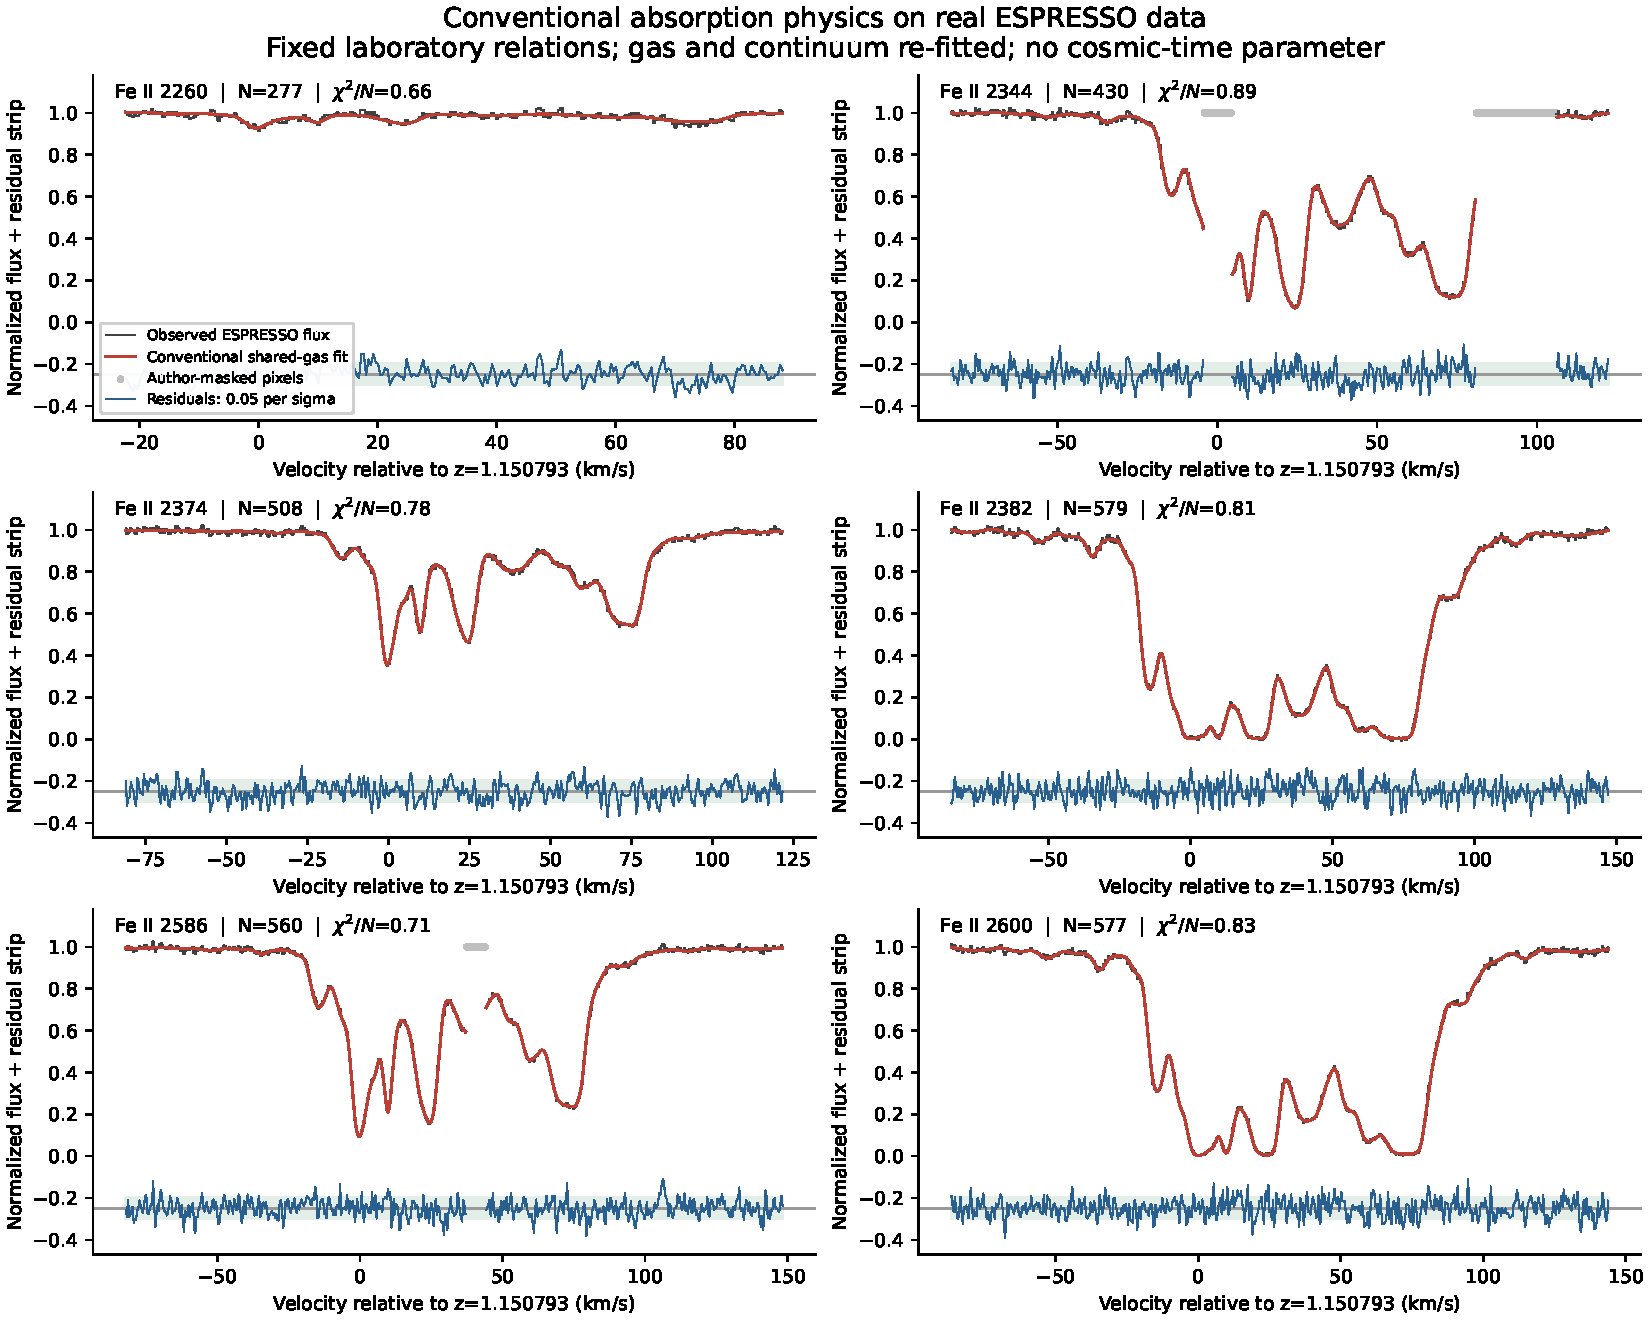
\includegraphics[width=.97\textwidth,height=.54\textheight,keepaspectratio]{espresso_conventional_null.pdf}
\caption{Joint conventional absorption fit to the six selected ESPRESSO Fe\,II transitions. The observed spectrum, model and residuals use the released masks and the same retained pixels. The lower strip in each panel displays normalized residuals, with one standard deviation corresponding to 0.05 on the plotted flux axis. Saturation, a shared multicomponent velocity structure, isotope sublines and instrumental convolution are included explicitly. This is a physical baseline test for one absorber, with no assumed inverse-logarithmic time response.}
\label{fig:espresso_null}
\end{figure}

This is an independent implementation using a subset of the published transitions, rather than an exact reproduction of the authors' multi-ion VPFIT analysis. Their final parameter file includes a freely fitted $\Delta\alpha/\alpha$; our $H_0$ explicitly fixes it to zero and refits the nuisance parameters. The primary weights use the archived normalized-error array. The separately supplied expected-fluctuation array defines a noise-sensitivity check, not a complete pixel covariance. Nominal parameter counts also do not remove degeneracies or boundary effects among closely spaced components.

Within each transition, the adjacent-pixel correlations of the fitted normalized residuals range from 0.31 to 0.46, excluding pairs across masked gaps. These empirical diagnostics can mix resampling covariance with remaining profile structure; they are not independent estimates of a complete noise model. They further preclude interpreting a diagonal-noise tail probability as a calibrated physical-discovery significance.

The initial robustness comparisons change the error array, assume an AR(1) pixel correlation of 0.3, perturb the instrumental width by $\pm3\%$, or remove the two transitions with published blend exclusions. These choices do not eliminate the conditional shift preference (Table~\ref{tab:espresso_null}). Subsequent exploratory checks, motivated by the strong-line pattern, allow relative opacity factors between 0.9 and 1.1 and zero-level adjustments of $\pm0.01$, or widen the gas-velocity and continuum bounds. These ranges are stress tests, not independently measured calibration priors. The preference remains. Removing 2382 and 2600 reduces the improvement to $7.09$ for three extra shifts, compared with $51.71$ for five shifts in the full set. This shows the importance of the strong lines while also discarding information; it does not identify a conventional mechanism that explains their offsets.

Independent implementations verify the opacity normalization, convolution and derivatives. A separate local analysis projects the shift derivatives against gas and continuum derivatives using singular-value decomposition. In 20,000 independent-Gaussian pixel simulations its five-dimensional score has mean 4.97 and variance 10.02. A $100\,\mathrm{m\,s^{-1}}$ shift injected into an exact forward spectrum is recovered as approximately $99.6\,\mathrm{m\,s^{-1}}$ by this local estimator. These checks establish numerical sensitivity under the stated model, not a calibrated discovery probability. The local score is distinct from the constrained nonlinear improvement; some unconstrained nuisance steps leave the allowed parameter ranges. A post-inspection blue/red velocity split shows compatible relative shifts under this same local approximation, so it does not isolate the effect to one side of the absorber. Global minima, full nuisance-model uncertainty and the true pixel covariance have not been established.

The component choice and masks were informed by these same observations, so this is not a blinded confirmation. Alternative gas structures, continuum and zero-level errors, instrumental-kernel errors, correlated noise, laboratory wavelengths and isotope abundances remain conventional explanations requiring further assessment. The improvement found here is evidence for residual transition inconsistency within a restricted model; it has not isolated a change beyond conventional explanations. One absorber cannot establish a temporal law: we infer no $1/\ln^2(t/t_*)$ amplitude, physical zero cutoff or accessible Riemann-zero height.

\subsection{Continuum covariance, saturated cores and an independent instrument}
\label{sec:espresso_followup}
% Generated from completed paired fits; see prepare_followup_manuscript.py.
\newcommand{\EspressoGLSDelta}{29.24}
\newcommand{\EspressoCoreOneDelta}{41.66}
\newcommand{\EspressoCoreThreeDelta}{13.26}

We next address three conventional limitations of the relative-shift comparison: correlated pixels, the strongest absorption cores and reproducibility in another instrument. These follow-ups were designed after inspecting the preceding results. They are exploratory sensitivity tests, with a fixed pixel set shared by $H_0$ and $H_1$ within each comparison, rather than independent confirmations of a physical change.

For a control outside the fitted absorption, we place 36 candidate continuum intervals at fixed velocity offsets from the six transitions, exclude the union of all 35 wavelength intervals listed in the authors' three published fit files, and assign overlapping pixels only once. Deterministic retention, median-flux and broad-feature criteria leave 25 disjoint intervals containing 13,750 pixels. We subtract a linear continuum in each interval without clipping individual residuals. Their adjacent-pixel correlation is $\widehat\rho_1=0.3726$, with a conditional 95\% interval $[0.3533,0.3916]$ from 10,000 resamples of whole intervals. The second-lag correlation is only $\widehat\rho_2=0.0440$, whereas an AR(1) model with this first-lag value predicts $0.1389$. Thus correlated residuals are present outside the absorption model, but a single AR(1) coefficient does not describe the measured correlation sequence (Fig.~\ref{fig:espresso_noise_controls}).

We therefore perform an additional constrained nonlinear generalized least-squares fit using the fixed correlation kernel
\begin{equation}
 R_{ij}=\begin{cases}
 \widehat\rho_k(1-k/11),&k=|n_i-n_j|\leq10,\\
 0,&k>10,
 \end{cases}
 \qquad C_{ij}=\sigma_i R_{ij}\sigma_j,
 \label{eq:espresso_control_covariance}
\end{equation}
where $n_i$ is the original pixel index and $\sigma_i$ the supplied error. Correlations therefore respect the actual separations across masked pixels; widely separated transition windows are treated independently. The taper regularizes the empirical sequence and is part of this specified sensitivity model. Both hypotheses re-optimize the gas and continuum parameters after Cholesky whitening. The resulting nonlinear improvement is $\Delta\chi^2=\EspressoGLSDelta$ for five additional shifts, compared with $51.71$ under diagonal errors. This is distinct from the earlier local projected score. The continuum residual variance is $0.7048$ times the supplied variance. Transferring this amplitude as well as the correlation shape would divide both objectives and their difference by $0.7048$, without changing their optima. We report that rescaling separately because the error variance in deep absorption need not follow the continuum. Neither covariance transfer nor its estimation uncertainty has been calibrated as a complete absorption-noise model.

\begin{table}[htbp]
\caption{Exploratory nonlinear ESPRESSO follow-ups, each adding five relative shifts. Each row compares the conventional model with relative transition shifts on the same retained pixels. The core exclusions use diagonal errors, separately from the full-pixel covariance fit; they are not a combined covariance-and-mask test. The reported improvements are conditional fit diagnostics, not calibrated discovery significances.}
\label{tab:espresso_followup}
\centering
\small
\begin{tabular}{lrrrr}
\hline
ESPRESSO comparison & Pixels & $\chi^2_0$ & $\chi^2_1$ & $\Delta\chi^2$ \\
\hline
Original diagonal errors & 2931 & 2305.49 & 2253.78 & 51.71 \\
Continuum-informed GLS & 2931 & 2231.33 & 2202.09 & 29.24 \\
Mask strong-line $F<0.1$ & 2692 & 2004.64 & 1962.98 & 41.66 \\
Mask $F<0.3$, pad 3 pixels & 2473 & 1722.96 & 1709.69 & 13.26 \\
\hline
\end{tabular}

\end{table}

To assess the strong cores without deleting the entire strong transitions, we freeze two masks from the preceding conventional model, before re-fitting either hypothesis. For 2382 and 2600 alone, we exclude model flux below 0.1, or below 0.3 with three additional native pixels on either side of each excluded run. The latter padding is $1.2\,\mathrm{km\,s^{-1}}$, obtained by rounding a requested $1\,\mathrm{km\,s^{-1}}$ upward on the $0.4\,\mathrm{km\,s^{-1}}$ grid. The resulting improvements are $\EspressoCoreOneDelta$ and $\EspressoCoreThreeDelta$, respectively (Table~\ref{tab:espresso_followup}). The masks do not follow noisy flux or move during optimization. Any weakening also removes velocity information, so it cannot by itself attribute the offsets to saturation or another particular mechanism.

The reported endpoints are bounded local solutions, selected after cross-starts and continuation of capped attempts. Stopping is primarily based on small relative objective changes; some nuisance parameters remain on bounds. These criteria do not certify a stationary point or a global minimum, and differences between recorded local solutions remain part of the numerical limitation.

\begin{figure}[htbp]
\centering
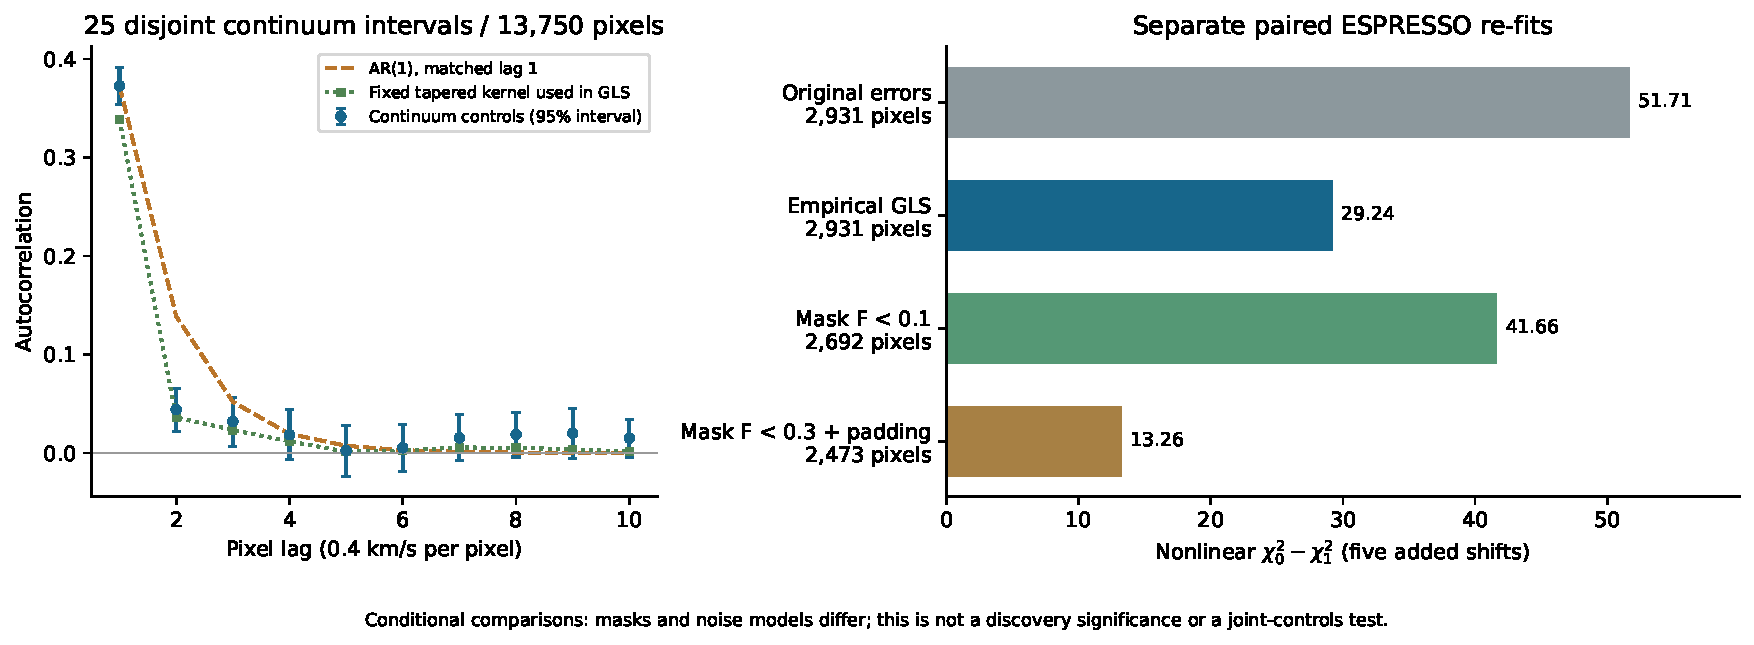
\includegraphics[width=.96\textwidth,height=.34\textheight,keepaspectratio]{espresso_noise_controls.pdf}
\caption{Continuum controls and subsequent nonlinear sensitivity tests. Left: the measured pixel autocorrelation, interval-resampling uncertainty, and the AR(1) and tapered empirical prescriptions. Right: improvements from adding the same five relative shifts in the original ESPRESSO comparison, the covariance re-fit and the two frozen core-mask re-fits. The covariance and masking changes are tested separately. These comparisons share the underlying observations and are not independent detections.}
\label{fig:espresso_noise_controls}
\end{figure}

For an instrument comparison we fit the UVES SQUAD coadd of the same absorber using 2374, 2382 and 2600, a shared 45-component gas model, and fitted continua, zero levels and Gaussian instrumental widths. The archived reduction log records exposure-dependent wavelength shifts and slopes; this coadd must not be described as wholly uncorrected. Its equivalence to the final precision product of a dedicated analysis, and its residual calibration uncertainty, remain unestablished. The nominal catalogue resolution gives an inadequate fit, while allowing the widths to vary substantially improves it. Integration is refined to 21 subpixels. The gas structure is poorly constrained, several parameters reach bounds, and the shift alternative reaches the allowed narrow-width boundary for 2374. At the saved endpoints, the two strong-line shifts are approximately $-0.14$ and $-0.13\,\mathrm{km\,s^{-1}}$, directionally compatible with ESPRESSO. The objective decreases are about 11.0 and 10.0 for two extra shifts under the statistical-error and expected-fluctuation arrays, respectively. Both null searches still reach their evaluation caps after a further 500 evaluations, so these differences are provisional rather than final likelihood-ratio estimates. An additional $\pm10\%$ relative-opacity control also remains optimization-limited. The comparison uses diagonal error arrays and remains conditional on this width and gas model. Independent photons do not make the shared component initialization or laboratory atomic data independent. This exercise does not independently establish the ESPRESSO relative shifts or a change in $\alpha$.

A recent route to a stronger test is HARPERFECT \cite{Milakovic2026HARPERFECT}, released as a preprint on 7 July 2026. It reprocesses approximately 52.5 hours of historical 2018 HARPS observations of this target, with explicit instrumental-response and sampling treatment. These are newly processed historical exposures. We did not locate downloadable science arrays and associated resolution matrices in the checked release channels, and therefore perform no HARPS re-fit here. Further independent calibration and gas-model checks remain necessary before asking whether any residual effect exceeds conventional explanations. None of these one-absorber comparisons identifies a cosmic-time law or an inverse-logarithmic amplitude.

\subsection{Combined controls and broader use of the available observations}
\label{sec:available_data}
% Generated from completed saved comparisons.
\newcommand{\JointCoreOneDelta}{23.69}
\newcommand{\JointCoreThreeDelta}{6.70}
\newcommand{\GasFortyDelta}{18.87}

We extend the conventional checks through combined covariance/core exclusions, a different gas architecture, individual ESPRESSO exposures and additional archived absorbers. These extensions follow inspection of the original target and are exploratory; the new-target screen uses declared quality criteria. Rules and intermediate endpoints are retained in the analysis records.

The combined controls apply the preceding frozen 2382/2600 core masks and tapered correlation kernel simultaneously. Covariance uses retained original pixel indices; both hypotheses re-optimize the same 45-component gas model and continua. Excluding model flux below 0.1 leaves 2692 pixels and gives $\Delta\chi^2=\JointCoreOneDelta$ for five added shifts. The wider exclusion, below 0.3 with three-pixel padding on either side, leaves 2473 pixels and gives $\Delta\chi^2=\JointCoreThreeDelta$ (Table~\ref{tab:available_data}). Improvements from different pixel selections cannot be combined into one likelihood-ratio statistic.

Masking also removes sensitivity. At the fixed diagonal-noise $H_0$ solution of Sec.~\ref{sec:espresso_null}, we project the shift derivatives against gas and continuum derivatives under the GLS weights. For the illustrative direction in which 2382 and 2600 each shift by $100\,\mathrm{m\,s^{-1}}$ while the other three relative shifts remain zero, the mild and wide masks retain approximately 70.5\% and 16.0\% of the full-pixel local information. This calculation ignores nuisance-parameter bounds and characterizes that single direction, not the marginal information for five free shifts. Thus the weaker wide-mask improvement cannot alone establish that saturation caused the original offsets.

\begin{figure}[htbp]
\centering
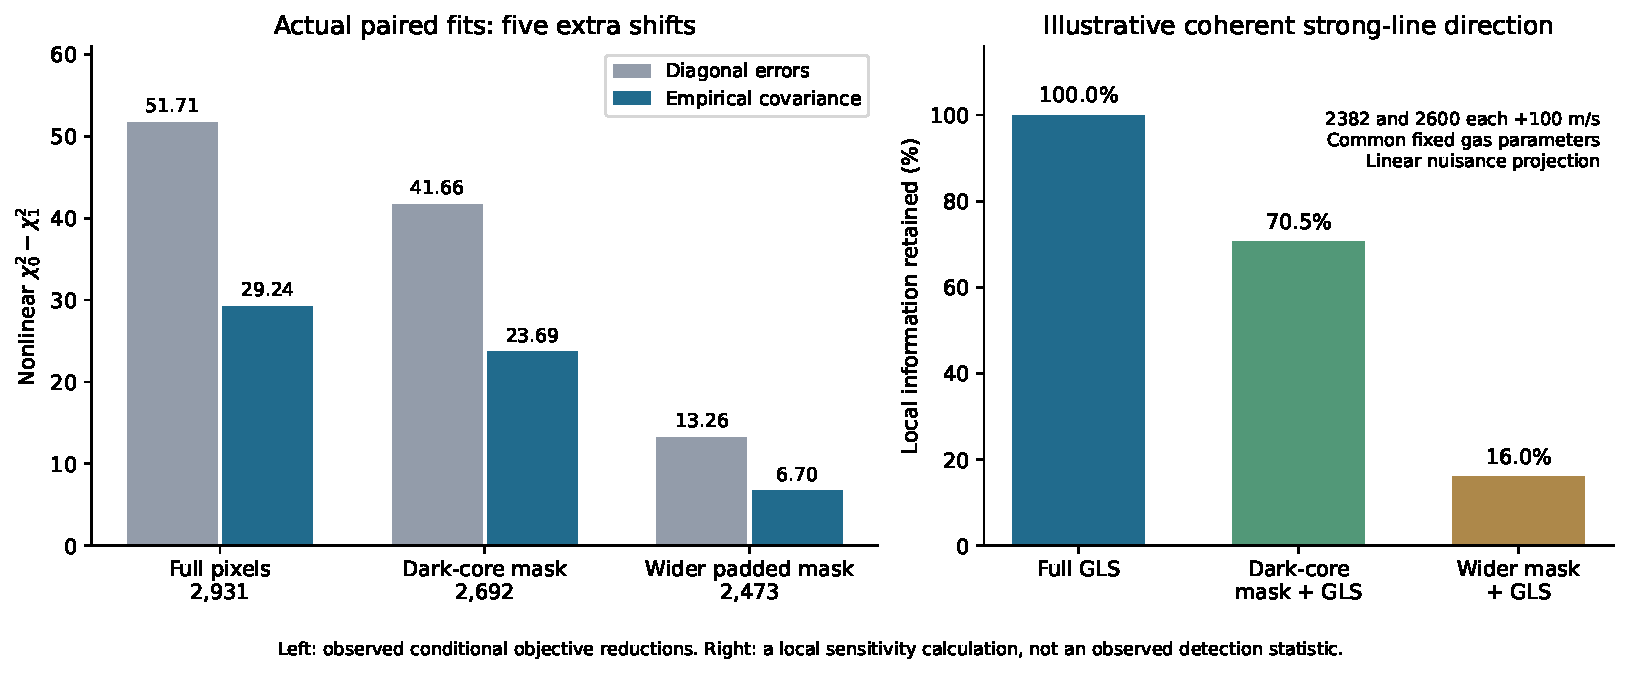
\includegraphics[width=.96\textwidth,height=.34\textheight,keepaspectratio]{joint_controls_information.pdf}
\caption{Combined controls and information removed by masking. Left: nonlinear improvements under diagonal and empirical GLS errors, each adding five shifts. Right: retained local information for one specified coherent strong-line shift, after nuisance projection at the fixed preceding baseline. This is conditional sensitivity, not evidence for a detected signal or all information in the data.}
\label{fig:joint_controls_information}
\end{figure}

We also replace the published 45-component architecture with a fixed 40-component alternative. Adjacent published component centres separated by less than $1.025\,\mathrm{km\,s^{-1}}$, half the smallest adopted instrumental FWHM, are joined into connected groups. Their initial total column density, column-weighted velocity and Doppler-core second moment are preserved; this does not preserve full Voigt profiles or assert that sub-resolution components are unmeasurable. Both hypotheses fit all 2931 pixels with the same empirical covariance, using 132 and 137 parameters. The original bound widths are centred on the merged initialization. The five-shift improvement is $\GasFortyDelta$, and the 2382 and 2600 shifts become approximately $-89$ and $-80\,\mathrm{m\,s^{-1}}$, changing by about $22\,\mathrm{m\,s^{-1}}$ from the 45-component GLS result. Two tested alternative-model starts terminate at objectives differing by $12.95$, so the selected local fit retains substantial initialization uncertainty. This tests sensitivity to a specified architecture and its bounds, not a nested statistical selection of the true number of clouds.

\begin{table}[htbp]
\caption{Combined masking/covariance controls and a gas-structure sensitivity test. Here $k_0$ counts the parameters of the conventional hypothesis. Each within-row comparison adds five relative shifts, using the same pixels, covariance and nuisance freedom. The empirical covariance retains the supplied variance amplitude. Results are bounded local fits; solver stopping criteria do not certify global minima. Cross-row objective differences are not independent discovery statistics.}
\label{tab:available_data}
\centering
\small
\begin{tabular}{lrrrr}
\hline
GLS comparison & Pixels & $k_0$ & $\chi^2_0$ & $\Delta\chi^2$ \\
\hline
Full pixels, 45 components & 2931 & 147 & 2231.33 & 29.24 \\
Joint $F<0.1$ mask + GLS & 2692 & 147 & 1931.90 & 23.69 \\
Joint padded $F<0.3$ mask + GLS & 2473 & 147 & 1684.36 & 6.70 \\
Full pixels, 40 components & 2931 & 132 & 2255.16 & 18.87 \\
\hline
\end{tabular}

\end{table}

For an exposure-level check, we retrieve all 17 extracted ESPRESSO S2D spectra and fit their native vacuum-barycentric pixel bins. The published exposure-specific rejections and atmospheric masks are transferred conservatively; no second barycentric correction is applied. This diagnostic fixes the gas template from the preceding combined-spectrum baseline while fitting line velocities and local continua and zero levels. The pooled shifts relative to 2374 are $-41.9\pm16.4$ and $-45.5\pm15.0\,\mathrm{m\,s^{-1}}$ for 2382 and 2600. Applying the same estimator to the combined spectrum gives $-42.8$ and $-39.6\,\mathrm{m\,s^{-1}}$. Agreement here checks two representations of the same observations; a full gas re-fit uses a different estimator. The shared data-derived template precludes an independent confirmation, and the quoted errors condition on that template and diagonal extraction errors.

The same 2600 transition appears in adjacent echelle orders. Its lower-index minus upper-index velocity is $-60.2\pm16.7\,\mathrm{m\,s^{-1}}$, or $-57.7\pm16.6\,\mathrm{m\,s^{-1}}$ when each order has a fitted Gaussian width; some free-width solutions reach their bounds. An order-dependent difference in the same physical transition directs attention to calibration, extraction, instrumental response and template approximations. It does not show that these effects explain the entire original offset, and its post-inspection conditional uncertainty is not a calibrated discovery test. Exposure-year comparisons likewise concern observational consistency, not a measurable change in the absorber's cosmic age.

Further UVES fits use expected-fluctuation errors and widen the Gaussian-width scale bounds from $[0.65,1.25]$ to $[0.5,1.4]$. The two strong-line shifts change by only $4$--$5\,\mathrm{m\,s^{-1}}$, while the 2374 width scale reaches $0.638$, below its former boundary. However, all four 1800-evaluation continuations and a 400-evaluation null cross-start fail the independently checked first-order stationarity criteria. Their finite objective differences therefore receive no calibrated significance. This symmetric-width control leaves covariance, calibration, non-Gaussian instrumental response and gas-model uncertainty unresolved; the independent photons still share gas architecture and atomic inputs with ESPRESSO.

The archive extension screens 155 identified damped Ly$\alpha$ absorbers along 132 sightlines within the 467-spectrum SQUAD archive \cite{Murphy2019SQUAD}. A coverage, forest, atmospheric-band and catalogue signal-to-noise screen selects 36 absorbers along 32 distinct sightlines under the initial atmospheric policy; broader water-band exclusions leave seven metadata candidates. All 32 spectra were retrieved and all 324 nine-transition windows analyzed. Six absorbers at $1.629\leq z\leq2.659$ pass the subsequent automatic coverage, noise and multiplet-detection criteria; three retain absorption-at-window-edge warnings. These are candidates for further modelling, not six calibrated precision measurements. The DLA catalogue is a targeted subset, not an exhaustive search for every Fe\,II absorber in 467 spectra, and systems on the same sightline share calibration.

We perform bounded Voigt-profile pilots for two compact candidate systems, selecting displayed component counts by exploratory $H_0$ AICc among 1, 2, 3, 4 and 6 components. In J232128$-$105122 at $z=1.629$, three shared gas components fitted to five transitions give conventional $\chi^2=80.59$ for nominal $\nu=101$; four additional shifts improve it by $6.84$. In J004131$-$493611 at $z=2.248$, six components and three transitions give $\chi^2=113.19$ for $\nu=108$, with an improvement of $5.66$ for two shifts. Both use the supplied statistical-error array with a diagonal covariance approximation; re-fitting with the archive's expected-fluctuation array gives improvements of $6.16$ and $5.50$, respectively. Component count and initialization matter: placing one shared component initially near a weak feature resolves an initially poor fit without increasing the number of components. These are initial model comparisons, not calibrated constant-variation measurements.

The 32 additional reduction logs contain no explicit nonzero exposure shift/slope entries; this does not prove that every calibration correction is absent. Wavelength distortions and gas structure require further assessment. Shared templates, atomic references and calibration assumptions also prevent treating all diagnostics as independent evidence. These extensions supply neither a calibrated $\Delta\alpha/\alpha$ measurement nor a homogeneous sample with a specified physical response for testing a cosmic-time law.


\subsection{Why this pilot does not identify a cosmic amplitude}
To connect spectra to the proposed schedule, an additional response could be posited as
\begin{equation}
 E_a(t)=E_a(t_0)+C g_a[h_2(t)-1],\qquad
 h_p(t)=\left[\frac{\ln(t_0/t_*)}{\ln(t/t_*)}\right]^p.
\end{equation}
Then $\Delta\nu=C(g_u-g_l)[h_2(t)-1]/h_{\rm P}$, where $h_{\rm P}$ is Planck's constant, with consistent coefficients for every shared level. The coefficients must be specified independently of the astronomical data. This deterministic level-shift assumption is additional to, and is not derived from, the standard-deviation component introduced earlier. Alternatively, a noise response needs its temporal correlation function and a line-shape calculation. A generic extra velocity width is degenerate with turbulence. No measured profile quantity here is automatically a constraint on $\delta_c$ or accessible zero height.

For a fixed candidate differential response $K_j$, a useful planning normalization is
\begin{equation}
 \Delta v_j(z)=K_jB G_2(z),\qquad
 G_p(z)=\frac{h_p(t(z))-1}{h_p(t(3))-1}.
 \label{eq:highz_response}
\end{equation}
Here $B$ has velocity units and $G_p(3)=1$. The accompanying calculations use a fixed flat matter-plus-$\Lambda$ background, $H_0=67.4\,\mathrm{km\,s^{-1}\,Mpc^{-1}}$ and $\Omega_m=0.315$, solely to assign ages; they do not fit cosmology. With the illustrative $t_*$ above, $h_2-1$ is 1.38\% at $z=1.1508$ and 2.72\% at $z=3.025$. These percentages describe the assumed component, not the fraction by which all atomic frequencies change.

For the initial two-sightline pilot, setting aside the high-redshift windows with telluric risk or inadequate noise quality leaves only 1608 as a candidate for further scrutiny. Even optimistically granting six usable low-redshift lines, these two spectra cannot identify $B$ when absorber redshifts and a constant response-mode offset $b_0$ are free. The single high-redshift line is absorbed by its redshift, while at the one remaining epoch $b_0$ and $B G_2$ are proportional. A numerical design-matrix example, using an artificial coefficient vector solely to illustrate this exact degeneracy, confirms unchanged rank when the cosmic column is added. This is an identifiability failure, not a zero-amplitude measurement. Therefore we report no best-fit cosmic coefficient, confidence limit on a cutoff, or preference for $p=2$ from this initial pilot. The subsequent archive expansion supplies additional multiplet candidates; their calibration, gas-model adequacy and the independently specified physical response still need to be established before a cosmic-time fit.

\subsection{Observations motivated by the measured limitations}
The actual profiles make the priorities more specific than a forecast based on independent identical lines. First, future targets should provide several common, sufficiently weak transitions over a range of absorber redshifts, with separate saturation and contamination checks. Second, exposure-level wavelength calibration, continuum and velocity-component modelling must be validated before a small formal offset is interpreted. Historical UVES/HIRES wavelength distortions motivate independent calibration and instrument comparisons \cite{WhitmoreMurphy2015}. The different transitions used at different redshifts must not silently redefine the response being tested.

Increasing exposure time alone is inefficient for the two poorest high-redshift windows. Even under the simplifying photon-noise law ${\rm S/N}\propto\sqrt{t_{\rm exp}}$, raising their full-window native-pixel ratios to 30 would require factors of about 523 and 211 in exposure, at unchanged observing conditions. These are relative arithmetic estimates, not observing-time requests, and do not remove telluric or blending errors. Selecting another target, another independently calibrated transition set, or more suitable near-infrared capability is therefore a substantive part of the design.

\begin{table}[htbp]
\caption{A staged program driven by the existing-data diagnostics. Durations and observing allocations are planning targets, conditional on staffing, sample yield and telescope availability. The primary deliverable is a validated constraint or a reproducible anomaly, not a guaranteed discovery.}
\label{tab:highz_roadmap}
\centering
\begin{tabular}{p{.16\textwidth}p{.42\textwidth}p{.34\textwidth}}
\toprule
Stage & Work & Criterion for useful progress\\
\midrule
Now--1 year & Archive screening; multicomponent fits; independent physical-response calculation; injections using realistic profiles & Freeze response and selection rules; verify bias and interval coverage before revealing a confirmation sample\\
1--3 years & Approximately 6--10 selected sightlines with present high-resolution facilities; an initial 50--200 h integration scenario, subject to object-level calculation & Obtain common line sets, calibration controls and independent instrument overlap\\
Later, within ten years & Expand independent sightlines and redshift coverage; use ANDES if commissioned and available & Recompute sensitivity using achieved performance; repeat any anomaly on held-out data\\
\bottomrule
\end{tabular}
\end{table}

The same six Fe\,II lines fit within ESPRESSO's nominal $380$--$788$\,nm coverage \cite{ESOESPRESSO2026} only over approximately $1.36<z_{\rm abs}<2.03$; a high-emission-redshift quasar does not automatically provide this line set at high absorber redshift. The ANDES team describes a baseline near $R=100{,}000$ over $0.4$--$1.8\,\mu$m and a 2035 first-light target \cite{NDiaye2026ANDES}. This is a conditional extension, not an achieved capability or guaranteed survey date. Existing facilities support the earlier stages independently.

In Eq.~\eqref{eq:highz_response}, the two pilot epochs have $\Delta G_2\simeq0.495$: an assumed $B=100\,\mathrm{m\,s^{-1}}$ corresponds to a response-mode difference of about $49.5\,\mathrm{m\,s^{-1}}$. This sets a conditional design scale, not a predicted or detected signal. Synthetic forecasts supplied with the project retain unknown response and systematic-floor assumptions. Even detecting such a trend would not automatically distinguish inverse-logarithmic exponents after amplitude and offset refitting. The appropriate progression is from a fixed physical response and validated measurement model to a blinded population test, with null results reported as limits on that specified response.


\section{What would test the proposal?}
A useful next experiment should separate preparation error, signal slope, decoherence, and estimator performance before introducing cosmic parameters. Repeated scans at fixed zero targets, with recorded interrogation duration, drive amplitude, shot count, and independent calibration, can test how ordinate uncertainty changes with the resource budget. Controls should include nearby nonzero targets and functions without zeta zeros. Known reference locations should be withheld from the inference stage where feasible, so that reproducing an encoded answer is not mistaken for discovering it. Scan boundaries and failed estimates must be reported alongside successful ones.

The relevant null model is a protocol-dependent conventional error budget with no additional aging component. A candidate excess term needs a specified response shared across apparatuses, a stable nuisance model, and out-of-sample predictions. A residual floor alone is insufficient: waveform imperfections and calibration errors also produce floors. An observed improvement after a hardware upgrade primarily tests the resource model. It becomes evidence for cosmic evolution only if the hypothesized time dependence can be separated from those changes.

At the illustrative microscopic scale used here, direct monitoring over months or years is unlikely to distinguish the proposed fractional evolution. Changing $t_\ast$ can make the slope larger, but then introduces a further parameter requiring independent justification. Cross-epoch observables could in principle provide greater leverage only if a physical mechanism connects their measurable quantities to the same uncertainty scale. Neither a reported variation of the fine-structure constant nor an error tolerance in prime reconstruction supplies that connection automatically.

There is consequently no present basis for preferring $p=2$ to a constant, $p=1$, $p=3$, or other sufficiently slow schedules using these two laboratory datasets. The exponent is retained because of its explicit theoretical motivation, while the proposed transfer from a map parameter to a physical uncertainty remains falsifiable only after a response model and an accessible precision target have been supplied.

\section{Limitations and conclusion}
The laboratory reanalysis uses rounded published estimates and author-processed coherence data. The astronomical extension uses historical coadded spectra, 17 native-pixel ESPRESSO exposures, and a targeted catalogue screen followed by 32 UVES spectra. The archive screen covers the 155 listed damped Lyman-alpha absorbers, not every metal absorber in SQUAD. The selected Fe II component decomposition, its parameter bounds and the missing full pixel covariance limit the interpretation of relative-shift preferences. The retrieved S2D arrays and reduction logs permit exposure diagnostics, but full extraction covariance, independently calibrated response matrices and complete calibration budgets have not been reconstructed in this work. Diagnostic groups and spectral intervals were selected for exploratory analysis and carry no confirmatory change-point or cosmic-evolution significance. The laboratory experiments use different protocols, and the mathematical reference computations here are not interval-certified. The cosmic extension has neither a measured amplitude nor an established identification of map iteration with physical age.

Within those limits, the empirical result is clear: the public trapped-ion summaries do not support a common abrupt breakdown at index 80, and the recent nuclear-spin work supplies an additional finite-resource implementation rather than evidence for a universal maximum zero height. A physical measurement has a protocol-dependent accuracy budget; a mathematical zero retains its exact definition. Accessible height can improve when an explicitly defined resource set improves. Extending this statement to cosmic age is a separate physical hypothesis. The inverse-log-squared form provides a concrete candidate for that extension, but current data do not establish its existence or superiority. This formulation leaves a tractable research program: characterize resource scaling, identify a reproducible residual component if one exists, and test a specified age dependence only when independent calibration makes that inference possible.

The additional spectroscopy analysis supplies measured absorption integrals, direct tests of profile sensitivity and a restricted conventional-model comparison. The latter finds residual transition inconsistency, especially in strong lines, that persists under several specified controls. It does not establish a variation beyond conventional explanations or a cosmic-age dependence. It shows why high signal-to-noise and a small formal fitting error are insufficient by themselves, and why usable common transitions at several epochs matter more than raw archive size. A future program can report constraints on a fixed atomic response, or independently reproduce an anomaly, without claiming to have measured a Riemann-zero cutoff. Establishing that stronger connection requires a separate physical derivation.

\section*{Data, code, and draft declarations}
The accompanying \texttt{riemann\_clock} project contains source provenance, public supplementary files, a pinned subset of the 2026 authors' repository, extracted data, analysis and figure scripts, and numerical validation reports. The original laboratory data are available through the cited publisher articles and the Wei et al. repository at \url{https://github.com/lqf2025/Riemann-data}, with the associated deposit \url{https://doi.org/10.5281/zenodo.20590665}. The astronomy extension includes two SQUAD source archives \cite{Murphy2019SQUAD}, NIST query snapshots, actual-profile measurements, registration diagnostics, a pinned public ESPRESSO spectrum and atomic/component inputs \cite{Murphy2022ESPRESSO}, joint Voigt null comparisons, disjoint continuum-noise controls, nonlinear covariance and frozen-core tests, an exploratory UVES instrument comparison, native-exposure/order diagnostics, additional SQUAD multiplet screening and physical-profile pilots, conditional injection controls, separately labelled synthetic forecasts, and a detailed experiment protocol. Third-party files retain their source provenance and applicable licenses. This study collects no human-participant or animal data.

The research hypothesis and source projects were supplied by Liang Wang. AI assistance was used for literature retrieval, source auditing, code preparation, numerical checking, and draft writing. This is an author-review draft; it does not assert completion of human review. Author contribution roles, current affiliation, funding, and competing-interest declarations remain to be finalized by the author before submission. No journal-specific compliance or external peer-review status is claimed.

\appendix
\section{Corrections to the exploratory construction}
The source notebooks do not fit a cutoff. One inserts a boundary at index 18.5, and another plots the assumed law
\begin{equation}
 T=\frac{\ln X}{\pi\sqrt{\epsilon}}.
\end{equation}
At $(X,\epsilon)=(10^{10},10^{-2})$ this gives $T=73.2936$, between the 18th and 19th ordinates. At $(10^{60},10^{-4})$ it gives $4397.61$. Neither calculation establishes a physical upper bound, and neither identifies a cutoff at the 80th zero. The free variables do not acquire a universal physical meaning from being displayed as a heatmap.

A sufficient truncation height for approximating a selected arithmetic function is a different quantity from a maximum experimentally accessible ordinate. Pointwise reconstruction errors depend on the function, smoothing, location relative to discontinuities, summation convention, and tolerance; exponential or monotonic convergence is not established by these notebooks. We do not infer a cosmological limit by identifying that reconstruction tolerance with a variation of an unrelated dimensionless constant.

The earlier waiting-time example is also internally inconsistent. Even under its unvalidated assumptions $X\propto t$ and $X\propto T^2$, changing an ordinate from 4200 to 4201 at $t_0=13.8$ Gyr would give
\begin{equation}
 \Delta t=t_0[(4201/4200)^2-1]=6.5722\ \mathrm{Myr},
\end{equation}
not 100 Myr. Using $\gamma_{4200}$ and $\gamma_{4201}$ instead gives $2.4694$ Myr under the same assumed scaling. These numbers are consistency checks, not replacement predictions. No waiting time is inferred in the revised framework.

Additional figures in the old source project were generated from piecewise synthetic error arrays with an imposed high-index deterioration. They are excluded from the empirical analysis. Every new experimental panel is traced to the primary supplementary table or the authors' processed experimental files; the conditional resource illustrations are labelled separately.

\bibliography{references,highz_references}
\end{document}
